\documentclass[12pt,a4paper,oneside]{book}

\usepackage[utf8]{inputenc}
\usepackage[style=numeric-comp, sorting=none]{biblatex}
\usepackage[english]{babel}
\usepackage{lmodern}
\usepackage{amssymb}
\usepackage{multirow}
\usepackage{amsmath}
\usepackage{txfonts}
\usepackage{mathdots}
\usepackage[top=1in, bottom=1in, left=1.1in, right=1.1in]{geometry}
\usepackage[autostyle]{csquotes}
\usepackage[font={small}]{caption}
\usepackage[classicReIm]{kpfonts}
\usepackage{graphicx}
\usepackage[colorlinks=true]{hyperref}
\usepackage{float}
\usepackage{array}
\usepackage{caption}
\usepackage{subcaption}


\addbibresource{ref.bib}


\newcommand{\eq}[2]{\begin{equation} \label{eq:#1} #2 \end{equation}}
        %\begin{document}
            %\eq{1}{x + y = z}
             %\eq{2}{a + b = c}
        %\end{document} 
\newcommand{\aeq}[2]{\begin{align} \label{eq:#1} #2 \end{align}}
\newcommand{\meq}[2]{\begin{multline}\label{eq:#1} #2 \end{multline}}
\newcommand{\seq}[2]{\eq{#1}{\begin{split} #2 \end{split}}}
\newcommand{\Eref}[1]{(\ref{eq:#1})}
\newcommand{\com}[1]{\textcolor{green}{ [Comment]: #1 }}


\title{
\sc
\Huge{Asymptotically flat vacuum solution for a rotating black hole in a modified  gravity theory}
\\[40pt]
\large{A Thesis submitted for the completion of}
\\[5pt]
\large{requirements for the degree of}
\\[15pt]
\Large{Bachelor of Science}
\\[5pt]
\Large{(Research)}
\\[20pt]
\normalsize{by}
\\[15pt]
\large{Arghya Ranjan Das}
\\[5pt]
\normalsize{Undergraduate Programme}
\\[5pt]
\normalsize{Indian Institute of Science}
\\[30pt]

\includegraphics[width=0.35\textwidth]{University_logo.pdf}
\\[40pt]
\normalsize{Under the supervision of}
\\[10pt]
\large{Prof. Banibrata Mukhopadhyay}\\
\normalsize{Department of Physics, Indian Institute of Science} \\[5pt]
\newpage
}


\author{}
\date{}
\begin{document}


\begin{titlepage}
\pagenumbering{gobble}
\maketitle
\end{titlepage}
\frontmatter


\chapter*{\centering Acknowledgements}
\addcontentsline{toc}{chapter}{Acknowledgements}
    \hspace{15pt} 
      I am forever indebted to my parents; their love and support have always encouraged me in all of my pursuits and inspired me to follow my dreams. They have always managed to handle their naughty child and gave him a fruitful environment for proper growth.
    
    I would like to convey my deepest gratitude towards my guide Prof. Banibrata Mukhopadhyay, for accepting to be the supervisor of my journey of Bachelor's thesis. Without his guidance, support, and helpful advice, this work could have never been a success. Besides being the supervisor, Prof. Banibrata Mukhopadhyay was also my lecturer for the physics lectures in Fundamentals of Astrophysics (2021) and my summer project advisor on accretion disks (2020). His approach to understanding and explaining physics has greatly enhanced my perception of getting deep insights and appreciation for the subject.
    
    I would like to thank the UG Physics coordinator, UG Dean, and the UG programme at IISc for allowing me to undertake such an excellent experience of a thesis project. I am grateful to KVPY, DST for the financial support received. I also want to thank Surajit Kalita, a fellow graduate student of my advisor, for sharing the codes of his work. I am thankful to my elder brother Archisman Panigrahi for various technical support and for always helping me in all aspects. Finally, I am grateful for the environment that IISc and its professors have offered and my friends for fruitful discussions and for never letting loneliness get to me. 





\newpage
\chapter*{Certificate}
This is to certify that the Bachelor’s thesis entitled \textit{``Asymptotically flat vacuum solution for a rotating black hole in a modified  gravity theory"}
submitted by Arghya Ranjan Das (Sr No. 11-01-00-10-91-18-1-15603) to Indian Institute of
Science, Bengaluru towards partial fulfilment of requirements for the award of the degree
of Bachelor of Science (Research) in Physics is a record of bona fide work carried out by
him under my supervision and guidance during academic year, 2021-22.
\begin{flushleft}
Date - 17$^{th}$ April, 2022 \\
Place - IISc, Bangalore           
\end{flushleft}
\hspace*{\stretch{1}}
$......................................................$ \\
\hspace*{\stretch{1}}
Prof.\ Banibrata Mukhopadhyay\\
\hspace{\stretch{1}}
\hspace*{\stretch{3}}
Department of Physics\\
\hspace{\stretch{1}}
\hspace*{\stretch{3}}
Indian Institute of Science\\
\hspace{\stretch{1}}


\chapter*{Declaration}
I, Arghya Ranjan Das, hereby declare that the material presented in the thesis titled \textit{``Asymptotically flat vacuum solution for a rotating black hole in a modified  gravity theory"} represents original work carried out by me in the \textit{Physics} department at \textit{Indian Institute of Science} during academic year, 2021-22, under the guidance of my
supervisor. This work has not been submitted to any other Institute for any degree or diploma. I have conformed to the norms and guidelines given in the Ethical Code of Conduct of the Institute and no unfair means have been used at any point in this project. Whenever I have used materials (data, theoretical analysis, figures, and text) from other sources, I have given due credit to them by citing them in the text of the thesis and giving their details in the references, and all the other images, tables, codes in this thesis are my own. 

\begin{flushleft}
Date - 17$^{th}$ April, 2022 \\
Place - IISc, Bangalore           
\end{flushleft}
\hspace*{\stretch{1}}
\hspace*{\stretch{3}}
$......................................................$ \\
\hspace*{\stretch{1}}
Arghya Ranjan Das\\
\hspace{\stretch{1}}
\hspace*{\stretch{3}}
Undergraduate Programme (Physics)\\
\hspace{\stretch{1}}
\hspace*{\stretch{3}}
Indian Institute of Science\\[2em]
\hspace{\stretch{1}}
\newpage




\chapter*{\centering Abstract}
\addcontentsline{toc}{chapter}{Abstract}
    \hspace{15pt}\noindent There are various ways to modify Einstein's gravity. The theory of $f(R)$ gravity is one of such modifications to gravity. In our present work, we  explore the vacuum solution of an asymptotically flat $f(R)$ gravity and establish a solution for rotating black hole, which is needed in various astrophysical contexts. Here we look at how modified gravity leads to a modified Schwarzschild solution and its rotating version being, essentially a modified Kerr solution. The solution exhibits a fundamental change in the properties of the black hole space-time like radii of marginally stable and bound orbits and black hole event horizon radius etc. Also, to look at the analytic version of this solution. We therein approximate the modification to be very small, and it is shown that the results of higher-dimensional branes are getting reproduced exactly. This signifies that the results of higher-dimensional branes are a special subset of this present work. It further argues for faster spinning black holes with spin (Kerr) parameter greater than unity, without the formation of any naked singularity. This supports the weak cosmic censorship hypothesis. 

{\hypersetup{linkcolor=black} \tableofcontents}
\mainmatter

\chapter{Introduction}
As the Newtonian theory of gravity fell short of explaining various astrophysical observations, Einstein's theory of general relativity (GR) became the most potent theory to replace the former. The general relativistic gravity of Einstein turned out to be a remarkable discovery that could explain a range of observational data, apart from its theoretical integrity, even after more than 100 years of its original discovery. It can well explain the properties of various compact objects such as black holes, neutron stars, white dwarfs, etc.\cite{Shapiro_Teukolsky_book}. This theory has been well tested through multiple experiments, which Newtonian theory could not explain, such as the bending of light rays, gravitational redshift, the perihelion precession of Mercury, etc. Eventually, all the predictions of Einstein's gravity came to be accurate, particularly after the detection of gravitational waves in 2015 \cite{GW15}.

Although GR is considered to be one of the successful theories, but several recent observations that it may fall short in very high-density regions \cite{0004-637X-517-2-565,1538-3881-116-3-1009,0004-637X-607-2-665}. For example, the observation of of peculiar type la supernovae (SNela) either with extremely high luminosity, inferred originating from white dwarfs of super-Chandrasekhar limiting mass as high as $2.8M_\odot$ \cite{2006Natur.443..308H,2010ApJ...713.1073S}  and extremely low luminosity , inferred from white dwarfs of sub-Chandrasekhar limiting mass as low as $0.5M_\odot$  \cite{1992AJ....104.1543F,1997MNRAS.284..151M,1998AJ....116.2431T,2001PASP..113..308M,2004ApJ...613.1120G,2008MNRAS.385...75T}. This gives a clear indication of violation of Chandrasekhar mass-limit (currently accepted value $\sim 1.4M_\odot$ for non-rotating, non-magnetized, carbon-oxygen white dwarfs  \cite{1931ApJ....74...81C}). Similarly, a number of neutron stars have been reported with a mass larger than $2M_\odot$ \cite{2018ApJ...859...54L,0004-637X-728-2-95}  are argued to be induced by modified Einstein's gravity \cite{2011JCAP...07..020A,2013JCAP...12..040A}. All these observations and inferences suggest that GR may not be the ultimate theory of gravity. Starobinsky was the first who overcame some of these shortcomings in cosmology through modified $f(R)$ gravity, where he considered second order in $R$ Ricci scalar. Eventually, various other models have been proposed to explain different aspects of astrophysical observations. Capozziello and his collaborators showed that by means of Starobinsky's $f(R)$ gravity and its higher-
order corrections, the problem of massive neutron stars could easily be explained \cite{2013JCAP...12..040A,2014PhRvD..89j3509A,2015JCAP...01..001A,2017CQGra..34t5008A,2016IJMPS..4160130A}. Similarly, Mukhopadhyay and his collaborators also showed that these models could also explain both the classes of the white dwarfs, viz. sub- and super-Chandrasekhar limiting mass white dwarfs which produce the peculiar SNeIa \cite{2015JCAP...05..045D,Kalita18}. 

However, to understand the coalescence of compact objects like black holes, neutron stars, etc., and to probe the underlying gravitational radiation, strong-field general relativity (GR) or numerical relativity is indispensable; most of the direct tests of GR are done based on weak field approximation. Thus the global validity of GR in a strong field, i.e., the true nature of gravity near the source, remains questionable, especially when the nature of such gravity is asymptotically flat. Asymptotic flatness assures the reduction of modified gravity to GR and ultimately to Minkowski space at a large distance from the source. Therefore, even if close to the source, i.e., compact objects like a black hole, neutron star, etc. the actual theory is modified gravity. The same theory will be able to explain any solar-system-based or earth-based experiments. Recently, Kalita and Mukhopadhyay have established asymptotically flat vacuum solutions of $f(R)$ gravity in spherical symmetry \cite{Kalita_Bani}, which essentially produces a modified Schwarzschild solution, hence non-rotating black holes. A brief discussion of this solution have been included in section \ref{Sec_non_rot_sol} and various properties of this space-time have been studied in \ref{Sec_Var_prop_non_rot}. This showed that various basic properties of the black holes like marginally stable and bound orbits, event horizons, etc., change depending on the modified gravity parameter. 

However, most cosmic objects are expected to rotate in general. The same goes for compact objects described by non-vacuum solutions. Thus a natural question arises on how the solution to GR modifies for rotating cases under modified gravity, especially under asymptotically flat modified gravity. In other words, how the Kerr solution change in modified $f(R)$ gravity?

This work establishes an asymptotically flat solution for rotating black holes in modified GR. Instead of deriving the solution from the appropriate modified action itself, we take a smooth alternative and rely on the Newman-Janis algorithm (NJA) \cite{NJA_Orig}. It can be shown \cite{NJA_1, NJA_Revisited} that various rotating solutions like Kerr solution, Kerr-Newman, etc. solution can be derived from the non-rotating version i.e. Schwarzschild solution, Reissner-Nordstorm metric, etc., respectively. The basic idea behind this is as if due to the choice of coordinates and metric parameters, the Kerr metric appeared to be diagonal and also spherical symmetric, like the Schwarzschild black hole. However, once the coordinates are expanded into actual coordinates with complex parts, it turns out to have off-diagonal terms with axial symmetry. We here applied NJA to the $f(R)$-gravity \cite{Kalita_Bani} to obtain the corresponding modified Kerr solution. Once we obtain the rotating solution, we explore various essential characteristics of the metric, e.g., the radius of the event horizon, marginally stable and bound circular orbits, various components of epicyclic oscillation frequency, orbital angular frequency, etc., with the change of black hole spin and modified gravity parameter.

The following work is organized as follows. In the chapter \ref{Chap_Modif_grav} the need of modification of gravity have been expressed following with basic formalism of $f(R)$ gravity in \ref{Sec_Basic_Form}; in the next section \ref{Sec_non_rot_sol} and \ref{Sec_Var_prop_non_rot}, we introduce the asymptotically flat vacuum solution that we kept under the consideration of this work and study the various properties of these solution. After that, we establish a rotating black hole solution in chapter \ref{Chap_Rot_Sol}  based on NJA. Further, we look at various properties of this space-time, such as the temporal and spatial components in section \ref{Sec_Temp_Rad_Rot_Sol} and discuss the nature of singularity of the metric and horizons in, respectively in section \ref{Sec_Source_Sing} and \ref{Sec_Hor}. We first present the numerical solution and then an approximate analytical solution for the horizon. Subsequently, we explore various fundamental orbits, as in GR, in this modified gravity framework for a test particle motion in section \ref{Sec_Orb} and corresponding fundamental oscillation frequencies in section \ref{Sec_Epi}. We conclude our work in section \ref{Chap_Conclude}
%===========================
\chapter{Modified $f(R)$ gravity}\label{Chap_Modif_grav}
In the last section, we looked at how observational mismatch with GR suggests modifying the present theory. However, even if one considers modification to GR is the way to go, it is not an easy task considering the numerous ways of deviating from GR. Many earlier attempts have been made to generalize Einstein's gravity, most of which have been shown to be non-viable \cite{Will:2018bme}. There are typical examples of numerous proposal to modified gravity in contemporary literature, namely, DGP (Dvali-Gabadadze-Porrati) gravity \cite{Dvali_2000}, brane world gravity \cite{Maartens_2004}, TeVeS (Tensor-Vector-Scalar) \cite{PhysRevD.70.083509} and Einstein-Aether theory \cite{PhysRevD.64.024028}. The subject of this present work is to look at modified $f(R)$ gravity specifically the asymptotically flat solution. The theories of $f(R)$ gravity comes about by a  straightforward generalization of the Einstein-Hilbert action. At this point one might question, why specifically $f(R)$ action and not more general ones, that include other higher-order invariants like $R_{\mu\nu}R^{\mu\nu}$ is not considered? This question can be addressed as \cite{Sotiriou_2010}, $f(R)$ actions are sufficiently general to encapsulate higher-order gravity and at the same time simple to handle with. Also, there are serious reasons to believe that $f(R)$ theories are unique among higher-order gravity theories, since they seem to be the only ones that can avoid long known and fatal Ostrogradski instability \cite{Woodard}.


\section{Basic formalism}
There are various modifications to Einstein's General relativity, $f(R)$ gravity is a family of modifications that considers the Ricci scalar $R$ in the Einstein-Hilbert action to be some arbitrary function of $R$. The simplest case of this is when the function is a constant, which gives the theory of General Relativity (GR). As a consequence of considering an arbitrary function, the choice of different functions can lead to the explanation of the accelerated expansion of the universe and structure formation without adding unknown forms of dark matter and dark energy. 

In GR, the Einstein-Hilbert action produces the Einstein's field equation through the principle of least action, which is given by \cite{Misner_Thorne_Wheeler_73}

\eq{EH_action}{S = \int \left[ \frac{c^4}{16\pi G}R + \mathcal{L}_M\right], }
where $c$ is the speed of light, $R$ is the scalar curvature (Often called Ricci scalar) such that $R = R_{\mu\nu}g^{\mu\nu}$, $G$ is the Newton's gravitation constant, $\mathcal{L}_M$ is the Lagrangian of the matter field and the integration is done on proper volume element. Varying this action w.r.t. $g_{\mu\nu}$ and equating it to $zero$ with appropriate boundary condition gives the Einstein's field equation for GR (interested readers can refer \ref{A_EF_Eq} for detailed calculation), given by
\eq{Field_eq}{G_{\mu\nu} = R_{\mu\nu}-\frac{1}{2}g_{\mu\nu}R = \frac{8\pi G}{c^4}T_{\mu\nu},}
where $T_{\mu\nu}$ is the energy-momentum tensor of the matter field. The equation \Eref{Field_eq} contains the information of the space-time on the L.H.S. and information about the matter in the R.H.S. which are related by this famous equation and shows that curvature in space-time and matter distribution are interrelated. In case of modified $f(R)$ gravity the Ricci scalar in equation \Eref{EH_action} is replaced by $f(R)$ (being an arbitrary function of $R$). The action is represented as
\eq{mod_action}{S = \int \left[ \frac{c^4}{16\pi G}f(R) + \mathcal{L}_M\right]. }
Now varying this modified action w.r.t $g_{\mu\nu}$ with appropriate boundary condition gives a modified version of the field equation, which is given by \cite{Felice_Tsujikawa_10, Nojiri_Odintsov_Oikonomou_17}
\eq{mod_Field_eq}{
F(R)G_{\mu \nu}+\frac{1}{2}g_{\mu \nu}[R F(R)-f(R)]-(\nabla_\mu\nabla_\nu-g_{\mu \nu}\Box)F(R) =\frac{8\pi G}{c^4}T_{\mu \nu},}
where $F(R) = \frac{d}{dR}f(R)$, $\Box$ is the d’Alembertian operator given by $\Box = \nabla^\mu\nabla_\mu$ and $\nabla_\mu$ is the covariant derivative. For $f(R) = R$, this equation reduces to the well-known Einstein field equation in GR.
Now considering a vacuum solution without any matter, the energy-momentum tensor vanishes, and equation \Eref{mod_Field_eq} reduces to
\eq{mod_Field_eq_vacuum}{
F(R)G_{\mu\nu}+\frac{1}{2}g_{\mu\nu}\left[R F(R)-f(R)\right]-\left(\nabla_\mu\nabla_\nu-g_{\mu\nu}\Box\right)F(R) =0.}
The trace of this equation takes the form 
\eq{Trace_eq}{RF(R)-2f(R)+3 \Box F(R) = 0.}
Substituting $f(R)$ from equation\Eref{Trace_eq} into equation \Eref{mod_Field_eq_vacuum}, we have
\eq{Trace_eq_2}{FR_{\mu\nu}-\nabla_\mu\nabla_\nu F = \frac{1}{4}g_{\mu\nu}\left(RF-\Box F\right).}
This equations \Eref{Trace_eq} and \Eref{Trace_eq_2} essentially completes the formalism to study the system, given we know the structure of $f(R)$ (or $F(R)$). Suppose we consider a spherically symmetric and static system in GR (i.e. with $F(R) = 1$) with the metric element as
\[g_{\mu\nu} =\mathrm{diag}\left(s\left(r\right),-p\left(r\right),\ -r^2,\ -r^2{{\mathrm{sin}}^2 \theta \ }\right)\]
Then from equations \Eref{Trace_eq} and \Eref{Trace_eq_2} we have \cite{Mut_Vij_06} 
\eq{1}{2\frac{X'}{X}+r\frac{F'}{F}\frac{X'}{X}-2r\frac{F''}{F}=\ 0}
\noindent and
\eq{2}{-4s+4X-4rs\frac{F'}{F}+2r^2s' \frac{F'}{F} +2rs\frac{X'}{X}-r^2 s' \frac{X'}{X}+2r^2\ s''=\ 0,} 
\noindent where $X\left(r\right)=p\left(r\right)s\left(r\right)$.
It can be seen that considering GR with $F(R) = 1$ the equation \Eref{1} leads to $X = \text{const}$, the const from Schwarzschild's solution can be found to be unity, and it can be also easily seen from equation \Eref{2} that the Schwarzschild's solution can be reproduced. \label{Sec_Basic_Form}

\section{Asymptotically flat solution}\label{Sec_non_rot_sol}

To get a asymptotically flat solution the $F$ must tend to $unity$ as the radial distance from the source $r\to \infty$, in which case we would recover the solution of GR and the model would pass tests like solar system test etc. Thus here we take a simple model with \cite{Kalita_Bani}
\eq{F_r}{F(r) = 1+\frac{B}{r},}
which we can see that as $r\to \infty$, $F(r)\to1$. Substituting equation \Eref{F_r} in equation \Eref{1} and solving for $X(r)$, we obtain
\eq{X_r}{X(r) = \frac{C_0r^4}{(B+2r^4)},}
where $C_0$ is a constant of integration. Now form the argument of asymptotic flatness as $r\to\infty$ we must have $s(r)\to1$ and $p(r)\to1$. Hence $X(r)\to1$ as $r\to\infty$, thus we have $C_0 = 16$. Therefore
\eq{ad}{X\left(r\right)=\frac{16r^4}{{\left(B+2r\right)}^4}.}
It is evident that setting $B=0$ (i.e. no modification to GR) we have $F(r) = 1$ and $X(r)=1$. Substituting equations \Eref{ad} and \Eref{F_r} in equation \Eref{2} and solving for $s(r)$ and expanding it in the power series of $r$, for $B\neq0$, we have
\meq{3}{
s\left(r\right)={} \frac{-16+2BC_1+32{\mathrm{log} 2 }+\left(BC_2+8\right)i\pi}{2B^2}r^2+1+\frac{B\left(-24+BC_2\right)}{24r}
	\\+\frac{B^2-\frac{1}{16}B^3C_2}{r^2}+\frac{-B^3+\frac{11}{160}B^4C_2}{r^3}+\frac{188B^4-13B^5C_2}{192r^4}+ \dots,}
where $C_1$ and $C_2$ are integration constants obtained by solving the second order differential equation \Eref{2}. Now as the metric should tend to Schwarzschild solution at large distance, thus we require the coefficient of $r^2$ to vanish and the coefficient of $1/r$ to be $-2$, which can be achieved by taking,
\eq{}{C_2=\frac{24\left(B-2\right)}{B^2},} 
\eq{}{C_1= -8\frac{B\left(-1+{\mathrm{log} 4 }\right)+\left(-3+2B\right)i\pi }{B^2}.}
Thus the temporal component of the metric is given by
\meq{4}{
g_{tt}=s\left(r\right)= 1-\frac{2}{r}-\frac{\left(-6+B\right)B}{2r^2}+\frac{B^2\left(-66+13B\right)}{20r^3}
-\frac{B^3\left(-156+31B\right)}{48r^4}\\+\frac{3B^4\left(-57+11B\right)}{56r^5}+O\left[r^{-6}\right]
}
and hence the radial component of the metric can be found as $g_{rr}=\ -p\left(r\right)$, where $p\left(r\right)=\ X(r)/s(r)$, and thus the power series solution takes the form as

\meq{5}{
p\left(r\right)= 1+\frac{2-2B}{r}+\frac{(-1+B)(-4+3B)}{r^2}-\frac{\left(-2+B\right)\left(80+B\left(-160+83B\right)\right)}{20r^3}
\\+\frac{16-52B+\frac{1}{60}B^2\left(3732+B\left(-1917+338B\right)\right)}{r^4}
\\+\frac{32-128B+\frac{1008B^2}{5}-155B^3+\frac{6002B^4}{105}-\frac{6431B^5}{840}}{r^5}\\+O\left[r^{-6}\right].
}
Moreover the Ricci scalar can be found to be
\meq{R}{R = \frac{3 B(-2+B)}{r^4}-\frac{3 B^2(-12+B)}{10 r^5}+\frac{B^3 (-51+8 B)}{10 r^6}-\frac{B^4 (-1776+293 B)}{280 r^7}\\+\frac{9 B^5 (-944+157B)}{1120 r^8}-\frac{B^6 (-3968+661 B)}{448 r^9}+\dots.}
which comes from the expression of $R(r)$ as \cite{Mut_Vij_06}
\eq{R_expr}{R(r) = \frac{2}{r^2p(r)}\left(1-p(r)+\left(\frac{s'(r)}{s(r)}-\frac{p'(r)}{p(r)}\right)\left(r-\frac{r^2s'(r)}{4s(r)}\right)+\frac{r^2s''(r)}{2s(r)}\right).}
\begin{figure}[t]
    \centering
    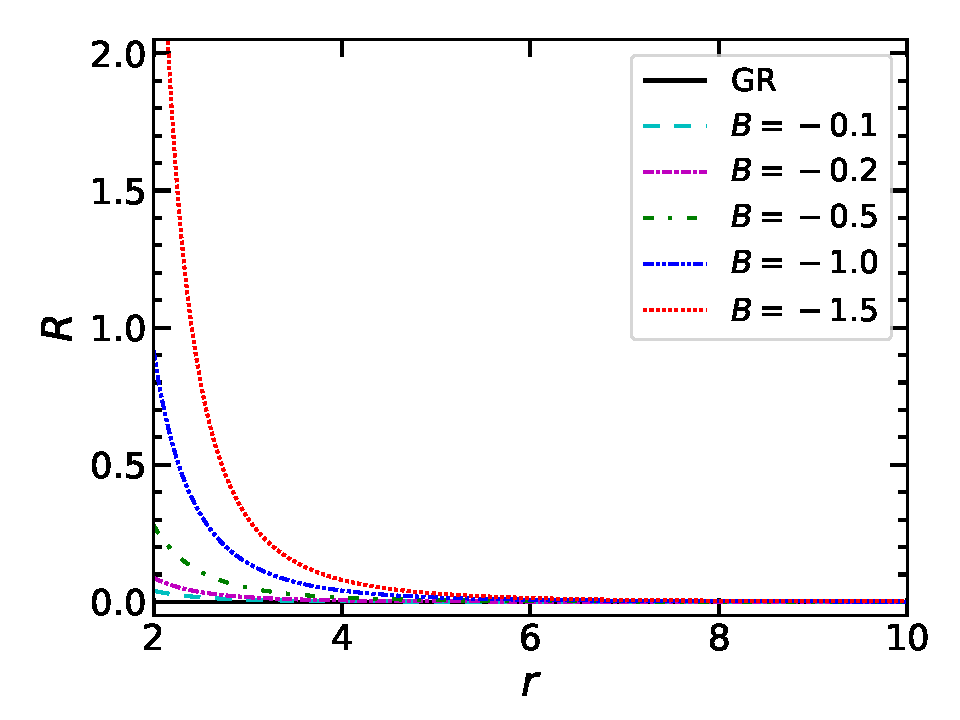
\includegraphics[width=0.7\textwidth]{Ricci.pdf}
	\caption{The variation of scalar curvature $R$ as a function of $r$ \cite{Kalita_Bani}.  }
        \label{Ricci}
\end{figure}
Now since $R$ has to be positive so that gravity can have its usual properties, i.e. it guarantees it is attractive, $B<0$ guarantees it. Now having found the expression of $R$, from equation \Eref{R} the $f(R)$ is given by,
\begin{align}
f(R(r)) &= \int F(R) dR \nonumber \\
&= \int F(r) \frac{dR}{dr}dr  \nonumber\\
&= \frac{3 B(-2+B)}{r^4}+\frac{3 B^2(-4+7B)}{10 r^5}+\frac{B^3 (-42+ 11B)}{20 r^6}\nonumber\\& \hspace{1.5cm}-\frac{B^4 (-552+101 B)}{280 r^7}+\dots  \\
\label{eq:f_R}
&= R+K_1R^{5/4}+K_2R^{3/2}+\dots \nonumber\\
&= R+\mathcal{O}(R^{>1}),
\end{align}
with $$K_1 = \frac{12}{5\times3^{5/4}}\frac{B^{3/4}}{(B-2)^{1/4}},\hspace{0.5cm} K_2=\frac{1}{60\sqrt{3}}\frac{B^{3/2}(B-12)}{(B-2)^{3/2}}.$$
This way in equation \Eref{f_R}, $f(R)$ is being expressed in terms of $R(r)$. In Starobinsky model, the $f(R)$ in Einstein-Hilbert action is considered to be $f(R) = R+R^2/6$ which is varying as $R^{1+1}$, whereas here it is varying as $R^{1+1/4}$. This difference from the Starobinsky model implies that the present theory of gravity has many astrophysical consequences and cosmological implicating, which will be discussed in the next sections.
It can be always verified that the putting $B=0$ or the case of large distance ($r\to\infty$) gives $F(r) = X(r) =1$ and in equations \Eref{4} and \Eref{5} gives back the Schwarzschild solution, given by
\eq{Sch_sol}{s(r) = 1-\frac{2}{r}, \hspace{0.5cm} p(r) = \frac{1}{1-\frac{2}{r}}}
along with $R=0$. Thus we see that this modified gravity theory produces a modified Schwarzschild metric which reduces to the Schwarzschild solution at large distance or if the modification is removed. This is the success of asymptotic flatness.

\section{Various properties of this asymptotic flat vacuum space-time}\label{Sec_Var_prop_non_rot}
In this section we will analyze the vacuum solution of asymptotic $f(R)$ gravity that we obtained in the last chapter and will discuss various physics lying with it. We will show that the property of this solution is very similar to the Schwarzschild solution and shows a similar trend.
%============================================================
\subsection{Temporal and spatial component of the metric}\label{Temp_rad_sec}
From figure \ref{temp_rad} the variation of temporal and radial components of the metric as a function of $r$ can be analyzed for various values of $B$. From the figure, it is evident that all the curves merge at a large distance, which implies that all of them tend to the Schwarzschild metric. However, this is not the case near the black hole; there is a significant deviation from the Schwarzschild solution at a smaller distance.
\begin{figure}[H]
	\begin{subfigure}[b]{0.5\textwidth}
         \centering
         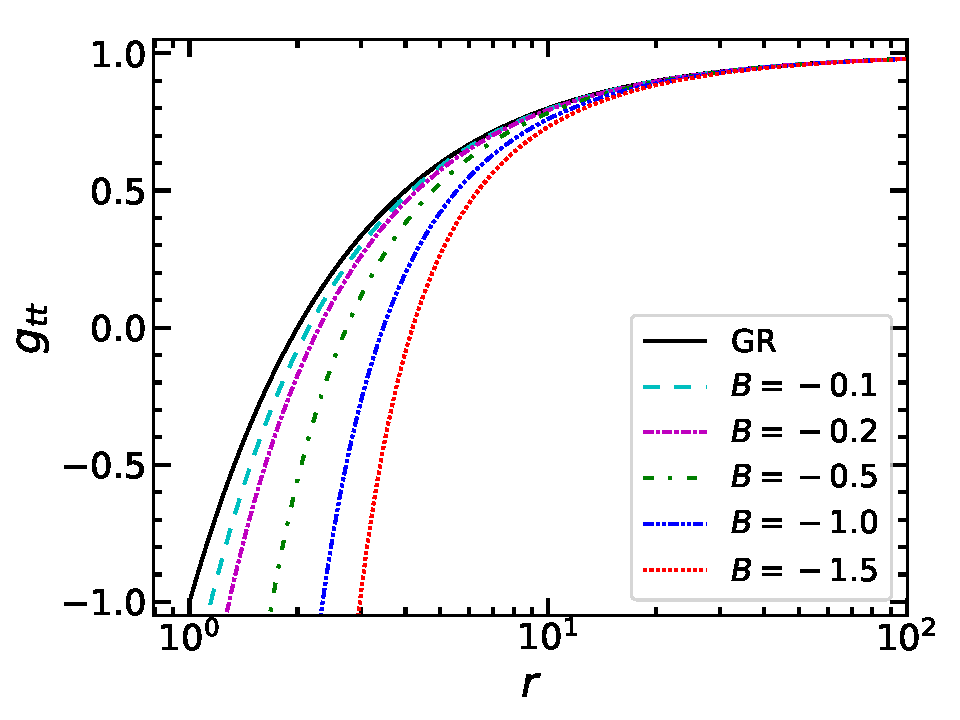
\includegraphics[width=\textwidth]{temporal.pdf}
	\caption{Temporal component ($g_{tt}$)}
    		\label{temporal}
     \end{subfigure}
    \hfill
     \begin{subfigure}[b]{0.5\textwidth}
         \centering
         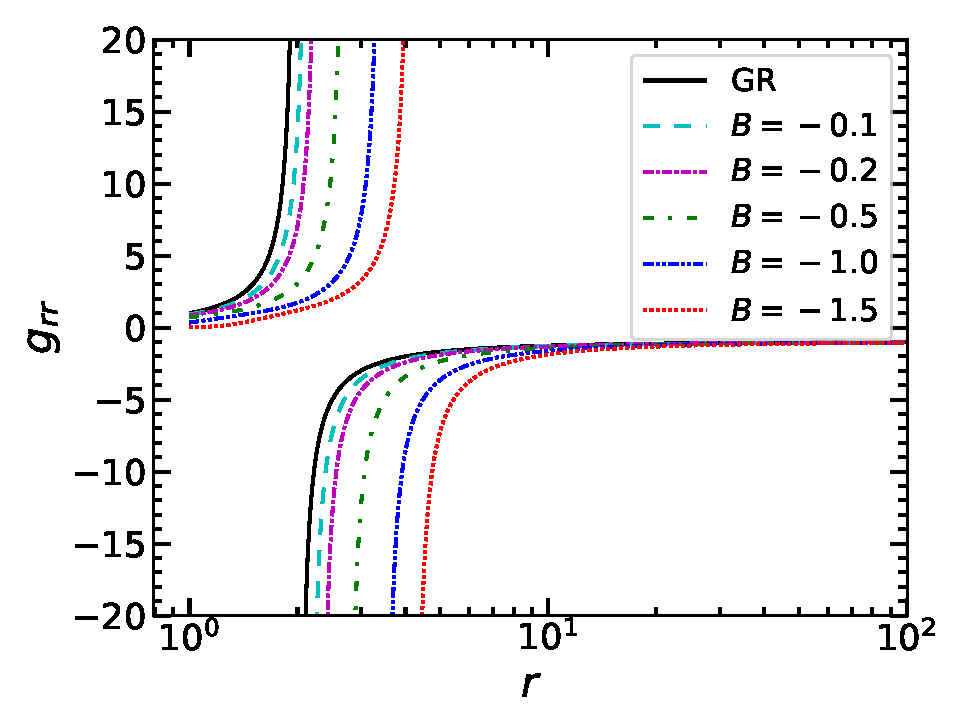
\includegraphics[width=\textwidth]{radial.pdf}
	\caption{Radial component ($g_{rr}$)}
    		\label{radial}
     \end{subfigure}
        \caption{Profile of temporal and radial element of the metric as a function of $r$ \cite{Kalita_Bani}.}
        \label{temp_rad}
\end{figure}
Noting from the radial component $g_{rr}$, it becomes divergent for some $r$, which is terms as the event horizon of the black hole. From figure \ref{radial}, we can see that with the increasing magnitude of $B$ the value of $r_H$ also increases. This confirms the impact of $f(R)$ gravity on the size of the black hole for the same mass s the Schwarzschild case. In GR, the size of a non-rotating black hole is completely determined by the mass $M$, whereas in the $f(R)$ gravity premise, even a non-rotating black's radius is determined by additional parameter(s), depending on the property of $f(R)$. 


%============================================================
\subsection{Marginally stable and bound orbits in $f(R)$ gravity}
In this section we will explore the various orbits of a test particle motion around the black hole. The conditions required for marginally stable circular orbit, marginally bound orbit can be found by defining an effective potential of the form
   \begin{figure}[!htbp]
     \subfloat[marginally bound\label{bound}]{%
     \centering
       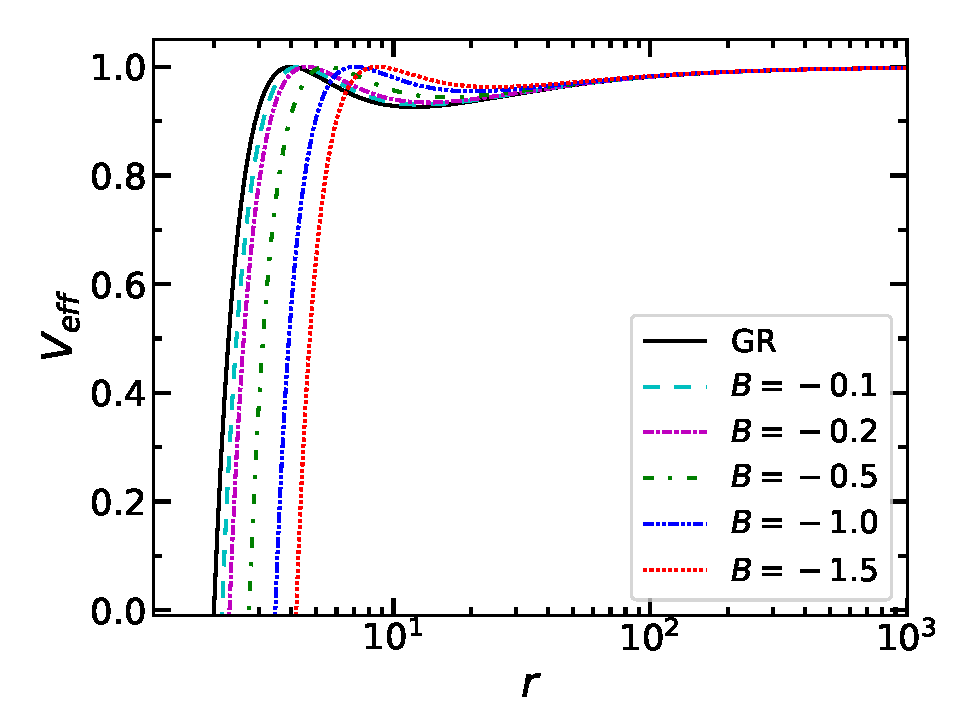
\includegraphics[scale = 0.5]{marginal_bound.pdf}
     }
     \hfill
     \subfloat[marginally stable\label{stable}]{%
     \centering
       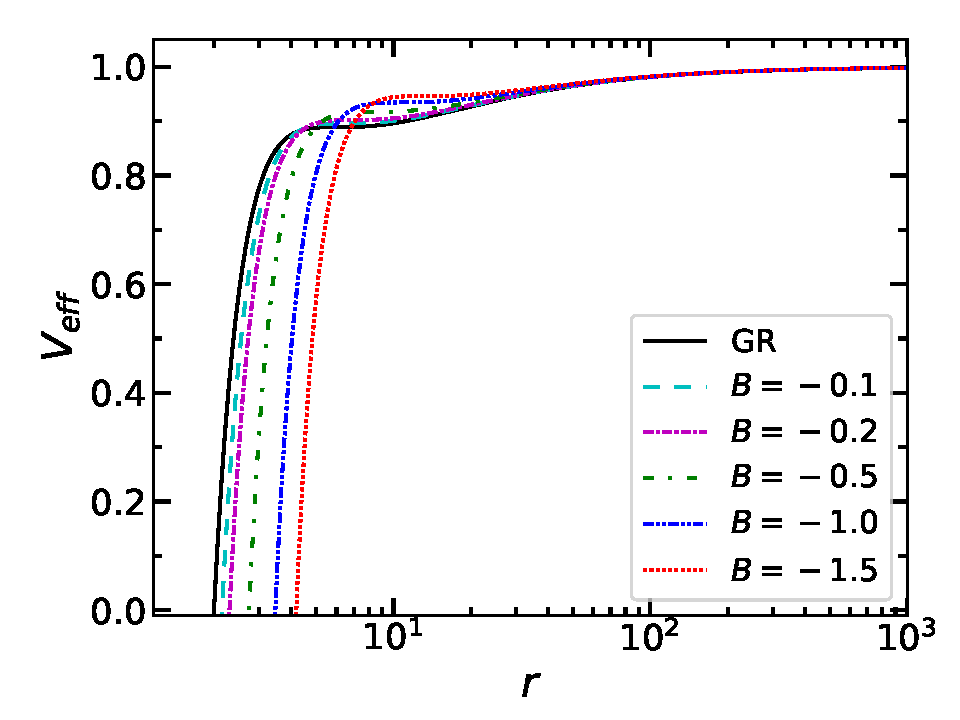
\includegraphics[scale = 0.5]{marginal_stable.pdf}
     }
     \caption{Effective potential for marginally bound and marginally stable circular orbits. All the quantities are expressed in dimensionless unit with $c=G=M=1$ \cite{Kalita_Bani}.}
     \label{marginal orbits}
   \end{figure}
\eq{}{V_{eff} = g_{tt}\left(1+\frac{L^2}{r^2}\right) ,}
where,
\eq{}{L = \sqrt{\frac{r^3\phi'(r)}{1-r\phi'(r)}},}
being the specific angular momentum of the particle.
Now the common conditions to obtain the equations to find the radial coordinate comes form the minimization of the effective potential. The other conditions are the marginal stability of the marginally stable circular orbits and marginal boundness of the marginally bound orbits. This conditions with the metric as $g_{\mu\nu}=\text{diag}\left(e^{2\phi(r)},-e^{2\lambda(r)},-r^2,-r^2\right)$ gives the equations to determine the marginally stable circular orbits and marginally bound orbits as,respectively,
\eq{}{1-e^{2\phi(r)}-r\frac{d\phi}{dr}=0}
\eq{}{3\frac{d\phi}{dr}-2r\left(\frac{d\phi}{dr}\right)^2+r\frac{d^2\phi}{dr^2}=0}
For convenience here, the assumption of $c=G=1$ has been made. Table \ref{parameters of space-time} shows the various marginal orbits for different values of $B$ and Figure \ref{marginal orbits} shows $V_{eff}$ for marginally bound and marginally stable circular orbits for various values of $B$. Here GR represents nothing but the results in the Schwarzschild space-time. It is interesting to note that as $B$ increases, $r_{H}$ increases, and, as a result, the radii of all the marginal orbits increase.

\begin{table}[!htp]
\centering
\begin{tabular}{|l|l|l|l|l|l|l|}
\hline
$B$ & $r_{H}$ & $r_{MB}$ & $r_{MS}$ & $r_{ph}$ & $L_{MB}$ & $L_{MS}$\\
\hline
GR & 2.00 & 4.00 & 6.00 & 3.00 & 4.00 & 3.46\\ 
-0.1 & 2.15 & 4.30 & 6.45 & 3.20 & 4.15 & 3.61\\ 
-0.2 & 2.30 & 4.60 & 6.90 & 3.40 & 4.29 & 3.75\\ 
-0.5 & 2.74 & 5.52 & 8.28 & 3.98 & 4.71 & 4.15\\ 
-1.0 & 3.47 & 7.07 & 10.64 & 4.94 & 5.37 & 4.78\\ 
-1.5 & 4.18 & 8.66 & 13.08 & 5.89 & 5.99 & 5.37\\ 
\hline
\end{tabular}
\caption{Various parameters of space-time for different values of $B$: $r_{H}$ is the event horizon, $r_{MB}$ the marginally bound orbit, $r_{MS}$ the marginally stable orbit, $L_{MB}$ and $L_{MS}$ are their corresponding specific angular momenta and $r_{ph}$ is the photon orbit. All the values are in dimensionless unit considering $c=G=M=1$. Data taken from \cite{Kalita_Bani}.}
\label{parameters of space-time}
\end{table}






%=========================================================
%=========================================================
\chapter{Rotating solution}
%=========================================================
%=========================================================
Until now, we have seen the non-rotating solution in modified gravity and how it affects different physical quantities. We found that depending on the modified gravity parameter, various characteristics of the black hole, like marginally stable and bound circular orbit, event horizon, etc., change. Also, we found that for a very hot accretion flow, critical/sonic point changes in modified gravity. 
However, in this cosmos hardly, we can find objects that are not rotating. Most of the cosmic objects are rotating, so a general black hole is expected to rotate. This leads to the requirement of a rotating asymptotically flat vacuum solution for this modified gravity. In this chapter, we devise the method to find the rotating solution.

%=========================================================
\section{Newman-Janis Algorithm(NJA)}

After the original discovery of the Kerr metric, Newman and Janis showed that the solution could be alternatively derived in a much easier fashion from the Schwarzschild solution by making an elementary transformation using complex numbers. In this method, the Schwarzschild was kept to be the "seed" metric, similarly, a new axisymmetric solution of the Field equation was derived using this method and was termed as Kerr-Newman metric, which is the solution of space-time around a charged rotating black hole.

In NJA during the complex transformation the spin parameter of the black hole comes into the solution as an arbitrary parameter. Now if we consider a static spherically symmetric metric then the line element could be written in the general form in $(+---)$ convention as \cite{Weinberg_1972} 
\eq{seed_line_element}{ds^2=s\left(r\right)dt^2-\mathrm{\ }p\left(r\right)dr^2-r^2\left(d{\theta }^2+{{\mathrm{sin}}^{\mathrm{2}} \theta \ }d{\phi }^2\right).}
\noindent In the null coordinates, this line element can be written, by 
advancing the time coordinate as $dt=du+\hat{f}dr$ and setting 
$\hat{f}=\pm {\left[s(r)/p(r)\right]}^{-\frac{1}{2}}$, as

%\eq{}{ds^2=s(r)\ du^2+2\ {\left[s\left(r\right)\ p\left(r\right)\right]}^{\frac{1}{2}}\ du\ dr -r^2\left(d{\theta }^2+{{\mathrm{sin}}^{\mathrm{2}} \theta \ }d{\phi }^2\right).}
\begin{eqnarray}
\nonumber
ds^2=s(r)\ du^2+2\ {\left[s\left(r\right)\ p\left(r\right)\right]}^{\frac{1}{2}}\ du\ dr\\ 
-r^2\left(d{\theta }^2+{{\mathrm{sin}}^{\mathrm{2}} \theta \ }d{\phi }^2\right).
\end{eqnarray}

\noindent Thus, the contravariant form of the metric can be written as

\eq{seed_metric}{g^{\mu \nu }=\left( \begin{array}{cccc}
0 & \ {\left[s\left(r\right)/ p\left(r\right)\right]}^{-\frac{1}{2}} & 0 & 0 \\ 
. & -\frac{1}{p\left(r\right)} & 0 & 0 \\ 
. & . & -\frac{1}{r^2} & 0 \\ 
. & . & . & -\frac{1}{r^2{{\mathrm{sin}}^{\mathrm{2}} \theta \ }} \end{array}
\right).}
Here ''$.$''s in equation \Eref{seed_metric} indicates that the metric is symmetric and will have corresponding elements as in the upper triangle. The contravariant form of the metric can then be expressed in terms of the null tetrads as \cite{NJA_Orig, NJA_1, NJA_Revisited}
\eq{null_tetrads_general}{g^{\mu \nu }=l^{\mu }n^{\nu }+l^{\nu }n^{\mu }-m^{\mu }{\overline{m}}^{\nu }-m^{\nu }{\overline{m}}^{\mu },} 

\noindent where the null tetrads satisfy the conditions

\eq{null_tetrads_general_cond}{
\begin{split}
   &l_{\mu }l^{\mu }=m_{\mu }m^{\mu }=\ n_{\mu }n^{\mu }=0,
   \\&l_{\mu }n^{\mu }=\ -m_{\mu }{\overline{m}}^{\mu }=1,
   \\&l_{\mu }m^{\mu }=n_{\mu }m^{\mu }=0,
\end{split}
}
with the bar(s) indicating the complex conjugates. 
Now from \Eref{seed_metric} the elements of the metric can be found and putting them into equation \Eref{null_tetrads_general}, along with equation \Eref{null_tetrads_general_cond}, the null tetrads are found to be
\eq{}{l^{\mu }={\delta }^{\mu }_1,}
\eq{22}{ n^{\mu }=\ -\frac{1}{2}\frac{1}{p\left(r\right)}{\delta }^{\mu }_1+\ {\left[s\left(r\right)\ p\left(r\right)\right]}^{-\frac{1}{2}}{\delta }^{\mu }_0,}
\eq{}{ m^{\mu }=\frac{1}{\sqrt{2}\ r}\left({\delta }^{\mu }_2+\frac{i}{{\mathrm{sin} \theta \ }}{\delta }^{\mu }_3\right).}
Then following NJA, we proceed by making a complex transformation as

\seq{}{
&u\to u'=u-ia \cos{\theta} \ ,
\\ &r\to r'=r+ia\cos{\theta},
\\ &\theta \to {\theta }'=\theta , 
\\&\phi \to {\phi }'=\phi.
}
This transformation can be considered as a complex rotation of the $\theta-\phi$ plane, the tetrads after the transformation thus becomes
\eq{}{l^{\mu }={\delta }^{\mu }_1,}
\eq{ad2}{n^{\mu }=\ -\frac{1}{2}\frac{1}{p\left(r,\theta \right)}{\delta }^{\mu }_1+{\left[s\left(r,\theta \right)\ p\left(r,\theta \right)\right]}^{-\frac{1}{2}}{\delta }^{\mu }_0,}

\eq{}{
	m^{\mu }=\frac{1}{\sqrt{2}\left(r+ia{\mathrm{cos} \theta }\right) }\left({ia{\mathrm{sin} \theta }\left(\delta ^{\mu }_0-{\delta }^{\mu }_1\right)+{\delta }^{\mu }_2+\frac{i}{{\mathrm{sin} \theta \ }}{\delta }^{\mu }_3}\right).
}
It should be hereby noted that the $s(r,\theta)$ and $p(r,\theta)$ in equation \Eref{ad2} are completely different from the $s(r)$ and $p(r)$ in equation \Eref{22} and are not necessarily equal. In fact the old functions are a function of only the radial coordinate $r$ whereas the new functions of both the radial $r$ and the angular $\theta$ coordinate.
From equation \Eref{null_tetrads_general}, the contravariant form of the metric is 
obtained as

\eq{}{g^{\mu \nu }=\ \left( \begin{array}{cccc}
-\frac{a^2{{\mathrm{sin}}^{\mathrm{2}} \theta \ }}{\mathrm{\Sigma }} & {\left[s\left(r,\theta \right)\ p\left(r,\theta \right)\right]}^{-\frac{1}{2}}+\frac{a^2{{\mathrm{sin}}^{\mathrm{2}} \theta \ }}{\mathrm{\Sigma }} & 0 & -\frac{a}{\mathrm{\Sigma }} \\ 
. & -\frac{1}{p\left(r,\theta \right)}-\frac{a^2{{\mathrm{sin}}^{\mathrm{2}} \theta \ }}{\mathrm{\Sigma }} & 0 & \frac{a}{\mathrm{\Sigma }} \\ 
. & . & -\frac{1}{\mathrm{\Sigma }} & 0 \\ 
. & . & . & -\frac{1}{\mathrm{\Sigma }{{\mathrm{sin}}^{\mathrm{2}} \theta \ }} \end{array}
\right),}

\noindent where $\mathrm{\Sigma }=r^2+a^2{\mathrm{cos}}^{\mathrm{2}} \theta$. The inverse of this metric, i.e. its covariant form, is



\eq{m1}{g_{\mu \nu }=\ \left( \begin{array}{cccc}
s\left(r,\theta \right) & {\left[s\left(r,\theta \right)\ p\left(r,\theta \right)\right]}^{\frac{1}{2}} & 0 & a{{\mathrm{sin}}^{\mathrm{2}} \theta \ }\left({\left[s\left(r,\theta \right)\ p\left(r,\theta \right)\right]}^{\frac{1}{2}}-s\left(r,\theta \right)\right) \\ 
. & 0 & 0 & -a\ {\left[s\left(r,\theta \right)\ p\left(r,\theta \right)\right]}^{\frac{1}{2}}{{\mathrm{sin}}^{\mathrm{2}} \theta \ } \\ 
. & . & -\mathrm{\Sigma } & 0 \\ 
. & . & . & -{{\mathrm{sin}}^{\mathrm{2}} \theta \ }\left(\mathrm{\Sigma }+a^2{{\mathrm{sin}}^{\mathrm{2}} \theta \ }\left(2{\left[s\left(r,\theta \right)\ p\left(r,\theta \right)\right]}^{\frac{1}{2}}-s\left(r\right)\right)\right) \end{array}
\right).}


\noindent Now we redefine the coordinates $u$  and $\phi$ such that, $du=dt+g\left(r\right)\ dr\ $and $d\mathrm{\phi }=d\varphi +h(r)\ dr$, with $g$ and $h$ as

\eq{}{g\left(r\right)=\ -\frac{(p{\left(r,\theta \right))}^{\frac{1}{2}}\left(\mathrm{\Sigma }+a^2{{\mathrm{sin}}^{\mathrm{2}} \theta {\left[s\left(r,\theta \right)\ p\left(r,\theta \right)\right]}^{\frac{1}{2}}\ }\right)}{{\left(s\left(r\right)\right)}^{\frac{1}{2}}\left(\mathrm{\Sigma }+a^2{{\mathrm{sin}}^{\mathrm{2}} \theta \ }e^{2\mathrm{\lambdaup }\left(r,\theta \right)}\right)},}

\eq{}{h\left(r\right)=\ -\frac{a\ p\left(r\right)}{\mathrm{\Sigma }+a^2{{\mathrm{sin}}^{\mathrm{2}} \theta \ }p\left(r\right)},}
In this new coordinate system, all the non-diagonal elements (excepts $g_{\phi t}$) goes to zero. This transforms the metric to Boyer-Lindquist coordinate system. Now putting $X(r,\theta) = p(r,\theta)s(r,\theta)$, the metric in this coordinate system takes the form as
\eq{6}{g_{\mu \nu }=\left( \begin{array}{cccc}
s\left(r,\theta \right) & 0 & 0 & a{{\mathrm{sin}}^{\mathrm{2}} \theta \ }\left({\left(X\left(r,\theta \right)\right)}^{\frac{1}{2}}-s\left(r,\theta \right)\right) \\ 
. & -\frac{\mathrm{\Sigma }}{\frac{\mathrm{\Sigma }\mathrm{\ }s\left(r,\theta \right)}{X\left(r,\theta \right)}\ +a^2{{\mathrm{sin}}^{\mathrm{2}} \theta \ }} & 0 & 0 \\ 
. & . & \mathrm{-}\mathrm{\Sigma } & 0 \\ 
. & . & . & -{{\mathrm{sin}}^{\mathrm{2}} \theta \ }\left(\mathrm{\Sigma }+a^2{{\mathrm{sin}}^{\mathrm{2}} \theta \ }\left(2{\left(X\left(r,\theta \right)\right)}^{\frac{1}{2}}-s\left(r\right)\right)\right) \end{array}
\right), }
which essentially leads to the counter part of rotating black hole of the metric in equation \Eref{seed_line_element}.


%=========================================================
\section{Transformation of specific functions under NJA}
With the knowledge of NJA, the angular momentum parameter can be easily incorporated into the non-rotating solution for the $f(R)$ gravity. In this section, we will look at how some specific functions transform under this complex transformation and hence ultimately find the rotating solution. However, when dealing with the complex transformation, we must note that since, in the end, we must have a real space-time hence the elements in the metric must remain real after the transformation. Now for a function $Q$ the transformation are given by \cite{NJA_Revisited,Source_and_singularity} \eq{Q_tran}{Q\left(r\right)\to Q\left(r,\overline{r}\right), }
Now since the functios $s(r)$, $X(r)$, $p(r)$, etc. all have terms involving with elements of the form $1/r^k$, thus the specific functions that we will keep in our considertion will be of the form $1/r^{2n}$ and $1/r^{2n+1}$ where $n$ is an integer. Now from transformation equation \Eref{Q_tran} and from the argument of getting a real function after transformation the function must be written as
\eq{}{\frac{1}{r^{2n}}\rightarrow \frac{1}{{\left(r\overline{r}\right)}^n},} 
\eq{}{\frac{1}{r^{2n+1}}= \frac{1}{r^{2n}}\frac{1}{r}\to \frac{1}{{\left(r\overline{r}\right)}^n}\frac{1}{2}\left(\frac{1}{r}+\frac{1}{\overline{r}}\right).}
Now suppose the function $Q\left(r,\overline{r}\right)$ has some terms of $\frac{1}{{\left(r\overline{r}\right)}^n}$ and $\frac{1}{{\left(r\overline{r}\right)}^{n}}\frac{1}{2}\left(\frac{1}{r}+\frac{1}{\overline{r}}\right)$ with at least one of them having a non-zero coefficient, then after the complex transformation of $u\to u'=u-ia \cos{\theta},\ \ r\to r'=r+ia\cos{\theta},\ \ \theta \to {\theta }'=\theta ,\ \ \phi \to {\phi }'=\phi$, the components of $Q\left(r,\overline{r}\right)$ will transform as

\eq{7}{\frac{1}{r^{2n}}\equiv \frac{1}{{\left(r\overline{r}\right)}^n}\to \frac{1}{\left[(r+ia\cos{\theta})(r-ia\cos{\theta})\right]^n}=\frac{1}{{\mathrm{\Sigma }}^n}}

\noindent and similarly

\seq{8}{&\frac{1}{r^{2n+1}}\equiv \frac{1}{{\left(r\overline{r}\right)}^n}\frac{1}{2}\left(\frac{1}{r}+\frac{1}{\overline{r}}\right)
\\&\hspace{1cm}\to \frac{1}{{\left[(r+ia\cos{\theta})(r-ia\cos{\theta})\right]}^n}\frac{1}{2}\bigg(\frac{1}{r+ia\cos{\theta}}+\frac{1}{r-ia\cos{\theta}}\bigg)\\&\hspace{1cm}=\frac{r}{{\mathrm{\Sigma }}^{n+1}},}
Thus, after the complex transformation, the function $Q(r)$ transforms to $Q(r,\theta )$.\footnote{$Q\left(r\right)$ and $Q(r,\theta)$ are not necessarily equal.}
Applying equations \Eref{7} and \Eref{8} to the functions $X\left(r\right)$, $s(r)$ and $p\left(r\right)$, we have 

\eq{9}{X\left(r,\theta \right)=\ \frac{{(r^2+a^2{{\mathrm{cos}}^{\mathrm{2}} \theta \ })}^2}{{\left({\left(\frac{B}{2}+r\right)}^2+a^2{{\mathrm{cos}}^{\mathrm{2}} \theta \ }\right)}^2},}

\meq{10}{s\left(r,\theta \right)=\ 1-\frac{2r}{r^2+a^2{{\mathrm{cos}}^{\mathrm{2}} \theta \ }}-\frac{\left(-6+B\right)B}{2\left(r^2+a^2{{\mathrm{cos}}^{\mathrm{2}} \theta \ }\right)}\cr+\frac{B^2\left(-66+13B\right)r}{20{\left(r^2+a^2{{\mathrm{cos}}^{\mathrm{2}} \theta \ }\right)}^2}
-\frac{B^3\left(-156+31B\right)}{48{\left(r^2+a^2{{\mathrm{cos}}^{\mathrm{2}} \theta \ }\right)}^2}\cr+\frac{3B^4\left(-57+11B\right)r}{56{\left(r^2+a^2{{\mathrm{cos}}^{\mathrm{2}} \theta \ }\right)}^3}+\dots,}

\meq{11}{p\left(r,\theta \right)=\ 1+\frac{(2-2B)r}{r^2+a^2{{\mathrm{cos}}^{\mathrm{2}} \theta \ }}+\frac{(-1+B)(-4+3B)}{r^2+a^2{{\mathrm{cos}}^{\mathrm{2}} \theta \ }}\cr-\frac{\left(-2+B\right)\left(80+B\left(-160+83B\right)\right)r}{20{\left(r^2+a^2{{\mathrm{cos}}^{\mathrm{2}} \theta \ }\right)}^2}
\cr+\frac{16-52B+\frac{1}{60}B^2\left(3732+B\left(-1917+338B\right)\right)}{{\left(r^2+{{\mathrm{cos}}^{\mathrm{2}} \theta \ }\right)}^2}
\cr+\frac{\left(32-128B+\frac{1008B^2}{5}-155B^3+\frac{6002B^4}{105}-\frac{6431B^5}{840}\right)r}{{\left(r^2+{{\mathrm{cos}}^{\mathrm{2}} \theta \ }\right)}^3}+\dots \ .}
Thus equations \Eref{6}, \Eref{9}, \Eref{10} and \Eref{11} essentially complete our development of the metric, which is the asymptotically flat vacuum solution for a rotating black hole in a modified gravity. It can be easily seen that by setting $B=0$, we obtain the usual Kerr-metric. Thus as expected, the usual GR solution is retrieved when the modified parameter is removed.
%=========================================================\l
\chapter{Looking at properties of the rotating\label{Chap_Rot_Sol} solution}\label{Chap_Var_prop__rot}
In the last chapter, we have completed the derivation of the rotating solution from the non-rotating metric in the modified gravity. Hereby in this chapter, we will analyze various properties of this space-time, like the profiles of the temporal and radial components, source and singularities, horizons, etc. From the discussion, we will see that this solution has a similar trend to the Kerr solution, which is a rotating solution in GR.
\section{Temporal and the spatial component} \label{Sec_Temp_Rad_Rot_Sol}
The variation of the temporal and the radial component of the metric have been shown in Figure \ref{TR four graphs}, for varying $B$ and $a$. The angle has been fixed in these profiles at $\theta = \pi/4$. From the figure, it is evident that all the curves merge at a large distance, which implies that all of them tend to Kerr solution at large $r$. But near the black hole, a significant deviation of the curves has been noticed. Figure \ref{temporal_var_B_a} and \ref{temporal_var_a_B} shows the variation of the temporal component $(g_{tt})$ for varying $B$ and $a$. It can be seen that for a fixed $a$, varying the $B$, the value of $g_{tt}$ at a given $r$ decreases with the increase in $|B|$. Whereas, when $B$ is kept fixed and the spin parameter $a$ is varied, then the value of $g_{tt}$ at a given $r$ increases with an increase in $|a|$. Looking at radial component $(g_{rr})$ in  Figure \ref{radial_var_B_a} and \ref{radial_var_a_B}, we can see that the location of the singularity varies with different values of $a$ and $B$, this have been analysed in the next section.

%%%% Image %%%% 
\begin{figure}[t]
	\begin{subfigure}[b]{0.5\textwidth}
         \centering
         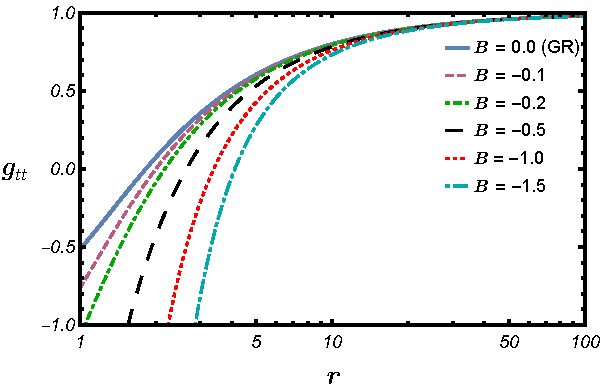
\includegraphics[width=\textwidth]{temporal_var_B_a.pdf}
	\caption{Temporal component $(g_{tt})$ for varying $B$}
    		\label{temporal_var_B_a}
     \end{subfigure}
    \hfill
     \begin{subfigure}[b]{0.5\textwidth}
         \centering
         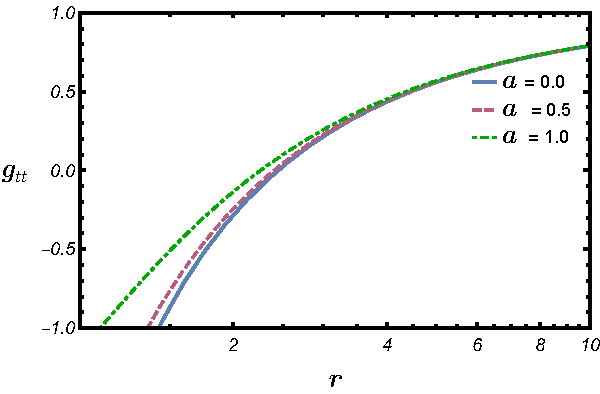
\includegraphics[width=\textwidth]{temporal_var_a_B.pdf}
	\caption{Temporal component $(g_{tt})$ for varying $a$}
    		\label{temporal_var_a_B}
     \end{subfigure}
     \newline
	\newline
     \begin{subfigure}[b]{0.5\textwidth}
         \centering
         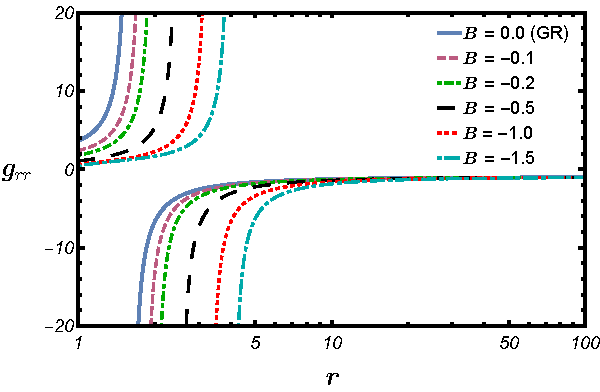
\includegraphics[width=\textwidth]{radial_var_B_a.pdf}
	\caption{Radial component $(g_{rr})$ for varying $B$}
    		\label{radial_var_B_a}
     \end{subfigure}
 \begin{subfigure}[b]{0.5\textwidth}
         \centering
         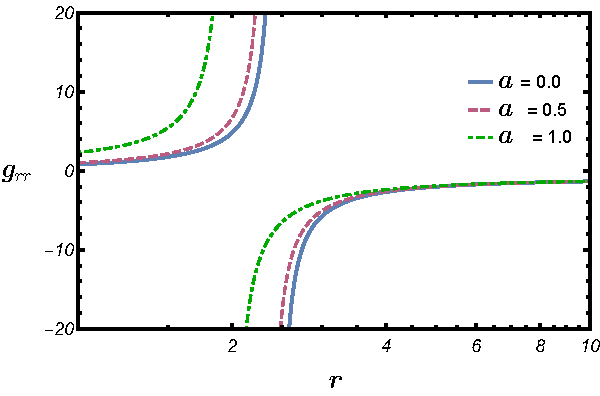
\includegraphics[width=\textwidth]{radial_var_a_B.pdf}
	\caption{Radial component $(g_{rr})$ for varying $a$}
    		\label{radial_var_a_B}
     \end{subfigure}
     \caption{Profiles of the temporal component $(g_{tt})$ and the radial component $(g_{rr})$ of the metric. Here the angle have been fixed at $\theta=\pi/4$, in (a) and (c) the spin parameter have been set to $a=0.8$, and in (b) and (d) the modified gravity parameter have been set to $B=-0.3$.}
        %\caption{Profiles of the Keplerian frequency $\nu_\varphi$ and the epicyclic frequencies $\nu_r$ (radial) and $\nu_\theta$ (vertical) in the modified theory with spin parameter set to $a = 0.8$. The modified gravity parameter $B$ has been set to 0.0, -0.3, -0.5, -1.0 in (a), (b), and (c). In (d) $B=0$ and -1.0 for bottom and top curves respectively for $\nu_\varphi$ and $\nu_\theta$,while for top and bottom curves for $\nu_r$.}
        \label{TR four graphs}
\end{figure}
\section{Source and singularity}\label{Sec_Source_Sing}
As we have found in section \ref{Temp_rad_sec}, in the non-rotating solution the radial part of the metric $g_{rr}$ was becoming divergent at some radius $r$. And from the knowledge of Kerr metric we expect a similar singularity in the rotating solution. From equation \Eref{6} we see that the metric becomes singular, when $s(r)$ or $p(r)$ becomes singular and that happens when $\mathrm{\Sigma }=0$, since $\mathrm{\Sigma }$ is present at the denominator in both. This shows that the metric becomes singular for \cite{Source_and_singularity}
\[r=0,\hspace{0.5cm} \theta =\frac{\pi }{2}.\] 
This singularity can be seen to be a geometric singularity by computing the curvature contraction $R_{\mu \nu \rho \lambda }R^{\mu \nu \rho \lambda }$. Further, it is an extended singularity, rather than `point -- like' singularity (as in Schwarzschild metric). 
Now transforming the coordinate to the Cartesian Minkowski coordinates can be done by,
\begin{align*}
    x =& r \sin{\theta} \cos{\phi} + \alpha \sin{\theta}\sin{\phi},\\
    y =& r \sin{\theta}\sin{\phi} -\alpha \sin{\theta}\cos{\phi},\\
    z =& r\cos{\theta},
\end{align*}
From this we immediately see that $r=0$ and $\theta =\frac{\pi }{2}$ corresponds to $x^2+y^2 = \alpha^2$ and $z=0$. Consequently, the physical singularity of the rotating solution is a ring singularity with the radius being $\alpha$. With small $B$ approximation, as we will see later the term involved with the spin angular momentum transforms as $\alpha \approx a + 1.5B$ (note when $B=0$ we have $\alpha = a$), thus the radius and the angular position of the singularity are, respectively,
\eq{12}{\alpha = a + 1.5B,\ \ \theta =\frac{\pi }{2}.}
\noindent Therefore, the singularity can be seen to be on a circle of radius $\alpha$ around the origin in the $z=0$ plane. The solution can be considered to lie uniformly distributed on this circle, bounding an interior disc $\sqrt{x^2+y^2}\le\alpha$. This singularity signifies the presence of a rotating black hole and is termed as ring singularity.


%=========================================================
\section{Horizons}\label{Sec_Hor}

In addition to the ring-like curvature singularity, there are also additional coordinate singularities. A suitable choice of coordinates can often remove such coordinate singularities, but they often underlie some important physical phenomenon and geometric description behind them. Considering the Boyer-Lindquist coordinates for the metric given by \Eref{6}, we define $\mathrm{\Delta }$ as

\eq{Horizon_cond}{\mathrm{\Delta }=\mathrm{\Sigma }\frac{s\left(r,\theta \right)}{X\left(r,\theta \right)}+a^2{{\mathrm{sin}}^2 \theta, \ }} 
thus the radial component is $g_{rr} = -\Sigma/\Delta$, which becomes singular when $\Delta = 0$. The solution of $r$ for $\Delta = 0$ gives two real values $r_\pm$ of which $r_-\leq r_{+}$. These radii are referred to as outer $(r_+)$ and inner $(r_-)$ horizons; the former is called the event horizon and the later one as the Cauchy horizon, and the region $r<r_+$ is referred to as the 'interior' of the black hole. It can be shown that the event horizon marks the point of no return. Now since $r_{-}$ lies inside the event horizon and no actual observer can have access to the interior of the event horizon, we avoid any discussion about the inner horizon $r_{-}$. 
%=========================================================
\subsection{Numerical Solution}
In previous section from equations \Eref{6}, \Eref{9}, \Eref{10} and \Eref{11}, the metric components have been obtained as a series solution and substituting $s(r,\theta)$ and $X(r,\theta)$ in equation \Eref{Horizon_cond} effectively gives $\Delta$, which depends on $r$, $\theta$, $a$ and the modified gravity parameter $B$. Due to the complexity off solving the problem, we restrict ourselves to the equatorial plane, $\theta = \pi/2$, and  opt to solve the equation to determine the radius of event horizon $r_H$ through numerical calculation. An simpler version of this problem have been solved analytically in the next section where we take a small $B$ approximation.
\begin{table}[t]
    \centering
\begin{tabular}{|p{0.15in}|p{0.3in}|p{0.3in}|p{0.3in}|p{0.3in}|p{0.3in}|p{0.3in}|p{0.3in}|p{0.3in}|p{0.3in}|p{0.3in}|p{0.3in}|p{0.3in}|} \hline
${\boldsymbol{r}}_{\boldsymbol{H}}$& \multicolumn{12}{|c|}{$\boldsymbol{a}$\textbf{}} \\ \hline
\multirow{12}{4em}{$\boldsymbol{B}$}&  & \textbf{0} & \textbf{0.1} & \textbf{0.2} & \textbf{0.3} & \textbf{0.4} & \textbf{0.5} & \textbf{0.6} & \textbf{0.7} & \textbf{0.8} & \textbf{0.9} & \textbf{1} \\ \cline{2-13}
 & \textbf{0} & 2.00 & 1.99 & 1.98 & 1.95 & 1.92 & 1.87 & 1.80 & 1.71 & 1.60 & 1.44 & 1.00 \\  \cline{2-13}
 & \textbf{-0.1} & 2.15 & 2.14 & 2.13 & 2.11 & 2.07 & 2.02 & 1.96 & 1.88 & 1.78 & 1.64 & 1.42 \\  \cline{2-13}
 & \textbf{-0.2} & 2.30 & 2.29 & 2.28 & 2.26 & 2.22 & 2.18 & 2.12 & 2.05 & 1.95 & 1.83 & 1.66 \\  \cline{2-13}
 & \textbf{-0.3} & 2.45 & 2.44 & 2.42 & 2.41 & 2.37 & 2.33 & 2.28 & 2.21 & 2.12 & 2.01 & 1.86 \\  \cline{2-13}
 & \textbf{-0.4} & 2.60 & 2.59 & 2.58 & 2.55 & 2.52 & 2.48 & 2.43 & 2.37 & 2.29 & 2.19 & 2.06 \\  \cline{2-13}
 & \textbf{-0.5} & 2.73 & 2.74 & 2.72 & 2.70 & 2.67 & 2.63 & 2.59 & 2.52 & 2.45 & 2.36 & 2.24 \\  \cline{2-13}
 & \textbf{-1} & 3.46 & 3.45 & 3.45 & 3.43 & 3.41 & 3.37 & 3.33 & 3.28 & 3.23 & 3.16 & 3.07 \\  \cline{2-13}
 & \textbf{-1.5} & 4.17 & 4.16 & 4.15 & 4.14 & 4.12 & 4.09 & 4.06 & 4.02 & 3.97 & 3.91 & 3.84 \\  \cline{2-13}
 & \textbf{-2} & 4.86 & 4.86 & 4.85 & 4.84 & 4.82 & 4.79 & 4.76 & 4.73 & 4.68 & 4.63 & 4.58 \\  \cline{2-13}
 & \textbf{-2.5} & 5.55 & 5.45 & 5.54 & 5.53 & 5.51 & 5.49 & 5.46 & 5.43 & 5.39 & 5.34 & 5.29 \\  \cline{2-13}
 & \textbf{-3} & 6.23 & 6.25 & 6.22 & 6.21 & 6.19 & 6.17 & 6.15 & 6.12 & 6.08 & 6.04 & 5.99 \\ \hline
 \end{tabular}
    \caption{Numerical values of $r_H$ for varying $B$ and $a$.}
    \label{Table1}
\end{table}

\begin{table}
    \centering
 \begin{tabular}{|p{0.15in}|p{0.3in}|p{0.3in}|p{0.3in}|p{0.3in}|p{0.3in}|} \hline
${\boldsymbol{r}}_{\boldsymbol{H}}$\textbf{} & \multicolumn{5}{|c|}{$\boldsymbol{a}$\textbf{}} \\ \hline
\multirow{12}{4em}{$\boldsymbol{B}$}& & \textbf{1.1} & \textbf{1.2} & \textbf{1.3} & \textbf{1.4}  \\ \cline{2-6}
 & \textbf{0} & - & - & - & - \\  \cline{2-6}
 & \textbf{-0.1} & - & - & - & - \\  \cline{2-6}
 & \textbf{-0.2} & 1.24 & - & - & - \\  \cline{2-6}
 & \textbf{-0.3} & 1.63 & - & - & - \\  \cline{2-6}
 & \textbf{-0.4} & 1.87 & 1.44 & - & - \\   \cline{2-6}
 & \textbf{-0.5} & 2.08 & 1.84 & - & - \\  \cline{2-6}
 & \textbf{-0.6} & 2.27 & 2.08 & - & - \\  \cline{2-6}
 & \textbf{-0.7} & 2.46 & 2.29 & 2.03 & - \\  \cline{2-6}
 & \textbf{-0.8} & 2.63 & 2.48 & 2.28 & - \\  \cline{2-6}
 & \textbf{-0.9} & 2.80 & 2.67 & 2.49 & 2.20 \\  \cline{2-6}
 & \textbf{-1} & 2.97 & 2.85 & 2.69 & 2.46 \\
\hline
\end{tabular}
    \caption{Numerical values of $r_H$ for varying $B$ and $a$, with $a>1$.}
    \label{Table2}
\end{table}



Tables \ref{Table1} and \ref{Table2} shows the variation of $r_H$ for different values of $B$ and $a$. We can thus observe that $r_H$ monotonically increases with the increase in $|B|$ for a fixed $a$ and decreases with increase in $a$ for a fixed $B$. From Table \ref{Table2} and Figure \ref{a_max_VS_B_Fig} it can be seen that unlike in kerr metric, $|a_{max}>1$ is allowed without the formation of any naked singularity due to $B<0$. The variation of maximum $a$, i.e. $a_{max}$, for varying $B$ is shown in Figure \ref{a_max_VS_B_Fig}.
%%%% Image %%%% 
\begin{figure}[H]
\centering
    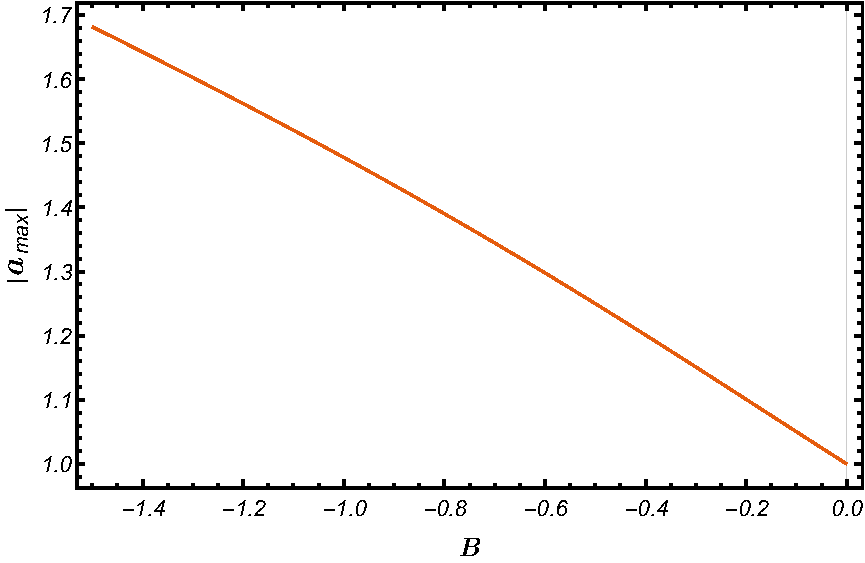
\includegraphics[width=0.7\textwidth]{a_max_VS_B.pdf}
    \caption{\centering Variation of maximum possible spin of black hole $a_{max}$ as a function of modified
	gravity parameter $B$.}
    \label{a_max_VS_B_Fig}
\end{figure}
%%%% Image %%%%
It can be seen from the Figure \ref{a_max_VS_B_Fig} that $|a_{max}|$ varies almost linearly with $B$. Exploring and interpreting these results with the exact solutions is beyond the scope of this work. We will look at an analytic approximation of the above feature and report the result in the next section, where we will calculate $|a_{max}|$. We will confirm that 
indeed $|a_{max}|$ is allowed to be greater than unity in modified gravity and also varies approximately linearly with $B$.
%=========================================================
\subsection{Analytical Approximation}
In order to assure the possibility of analytic solution, we consider the modification to GR to be very Small hence we take $B\ll1$. Thus we take only terms upto $r^{-2}$, thus the functions $s(r,\theta)$ and $p(r,\theta)$ can be written as
\eq{app_s_r_theta}{
	s\left(r,\theta \right)=\ 1-\frac{2r}{r^2+a^2{{\mathrm{cos}}^{\mathrm{2}} \theta \ }}-\frac{\left(-6+B\right)B}{2\left(r^2+a^2{{\mathrm{cos}}^{\mathrm{2}} \theta \ }\right)}+O[r^{-3}],}

\eq{app_p_r_theta}{p\left(r,\theta \right)=\ 1+\frac{(2-2B)r}{r^2+a^2{{\mathrm{cos}}^{\mathrm{2}} \theta \ }}+\frac{(-1+B)(-4+3B)}{r^2+a^2{{\mathrm{cos}}^{\mathrm{2}} \theta \ }}+O\left[r^{-3}\right].}
Taking terms upto $r^{-2}$, in Boyer-Lindquist coordinate system, the metric can be recast from equations \Eref{6}, \Eref{app_s_r_theta}, \Eref{app_p_r_theta} and taking further $B\ll 1$ and having $X\approx1$, the nonzero component of the metric comes out to be

\eq{}{g_{\mu \nu }=\left( \begin{array}{cccc}
1-\frac{2r}{\mathrm{\Sigma }}-\frac{\beta}{\mathrm{\Sigma }}& 0 & 0 & \frac{2a{{\mathrm{sin}}^{\mathrm{2}} \theta}}{\Sigma}(2r+\beta) \\ 
. & -\frac{\mathrm{\Sigma }}{\Delta} & 0 & 0 \\ 
. & . & \mathrm{-}\mathrm{\Sigma } & 0 \\ 
. & . & . & -{{\mathrm{sin}}^{\mathrm{2}} \theta \ }\left( r^2 + a^2 +  \frac{a^2\sin{\theta}(2r+\beta)}{\Sigma}\right) \end{array}
\right),}
\noindent where $\Delta \approx r^2 + a^2 -2r -\beta$, and $\beta=\left(-6+B\right)B/2\approx-3B$. \footnote{Note, $B\le 0\to \beta\ge 0$ as $B=-\beta/3$.}
Thus the line element is of the form
\meq{brane_line_element}{ds^2 = \left(1-\frac{2r}{\mathrm{\Sigma }}-\frac{\beta}{\mathrm{\Sigma }}\right) dt^2 + \left(\frac{4a{{\mathrm{sin}}^{\mathrm{2}}  \theta}}{\Sigma}(2r+\beta)\right) dt d\varphi 
\\-\frac{\Sigma}{\Delta}dr^2 - \Sigma d\theta^2 -{{\mathrm{sin}}^{\mathrm{2}} \theta \ }\left( r^2 + a^2+ \frac{a^2\sin{\theta}(2r+\beta)}{\Sigma}\right)d\varphi^2 .}
Observing the line element equation \Eref{brane_line_element}, it can be seen that this line element matches exactly with the results of vacuum solution from consideration of higher-dimensional branes \cite{Charged_BH_Brane, BH_Brane}. This result is quite marvelous as this shows that the work presented here already includes the results of higher-dimensional branes. The results of higher-dimensional branes comes as a special solution of the present theory with the small $B$ approximation and hence can be considered as a subset of the present work.

Now to find the horizon for this case, we will have to find $\Delta$ from equation \Eref{Horizon_cond} and equate $\Delta = 0$. After approximation the $\Delta$ can be found to be 

\eq{}{\mathrm\Delta={\Sigma }\left(1-\frac{2r}{\mathrm{\Sigma }}-\frac{\beta}{\mathrm{\Sigma }}\right)+a^2{{\mathrm{sin}}^2 \theta \ }\approx0,}


\noindent which gives
\begin{equation}
\Delta=r^2-2r+\left(a^2-\beta\right)=0.
\label{Del}
\end{equation}

\noindent Thus, to the first order in $B$, we obtain $\mathrm{\Delta }=r^2+a^2-2r-\beta$. Now solving the quadratic equation (\ref{Del}) gives two three-surfaces of constant $r$ as
\[r_{\pm }=1\pm \sqrt{1-\left(a^2-\beta \right)}.\] 
These surfaces give the outer $(r_+)$ and inner $\left(r_-\right)$ horizons. Thus, the event horizon takes the form as
\eq{13}{r_H=r_+=1+\sqrt{1-a^2+\beta}.}
%%%% Image %%%% 
\begin{figure}[t]
\centering
    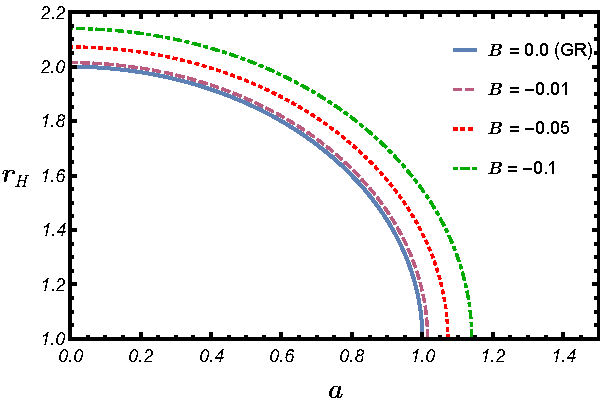
\includegraphics[width=0.7\textwidth]{Analytic_r_H_Vs_a_fixed_B.pdf}
    \caption{\centering Analytic solution for $r_H$ with the change of $a$ for different $B$.}
    \label{fig:1}
\end{figure}
%%%% Image %%%%


It can be easily seen that the event horizon in a Kerr metric can easily be recovered by setting $B=0$, $r_{H_0} = 1+\sqrt{1-a^2}$ This suggests the validity of the analytic solution. Figure \ref{fig:1} shows the trend of $r_H$ w.r.t $a$ for various modified gravity parameter $B$. Matching with Table \ref{Table1} can be seen that for $a=0$ the results match quite well with the analytic result presented here. However, as $|B|$ increases the results to deviate significantly, which is because the higher terms in $s(r,\theta)$ and $p(r,\theta)$ becomes dominant. Quantittively, wen $B\approx-0.1$, very small compared to $r$, the numerical reulst s matches quite well with the approximate analytical solution; thus, the analytical approximation is valid for $B\ge-0.1$ regime, so that 
\[{\left(r_{H_{analytical}}\right)}_{B\ge -0.1}\approx {\left(r_{H_{numerical}}\right)}_{B\ge -0.1}.\] 
From equation \Eref{13}, for $r_H$ to be real we must have
\[1-\left(a^2-\beta \right)\ge 0,\] 
\[\to \left|a\right|\le \sqrt{1+\beta }.\]
Thus,
\eq{a_max_eq}{|a_{max}| = \sqrt{1+\beta },}
\eq{approx_a_max_eq}{|a_{max}|\approx 1 + \beta/2 \approx1-1.5B\geq|a_{max}|_{_{kerr}}.}
From equation \Eref{a_max_eq} the maximum value of $|a_{max}|$ obtained to be different from that obtained from Kerr metric and because $\beta \geq 0$, black holes can have spin parameter of value more than unity, i.e. $\left|a\right|\ge 1$, without the formation of any naked singularities. The linear dependence of spin on modified gravity parameter can also be seen from equation \Eref{approx_a_max_eq} which nearly matches with Figure \ref{a_max_VS_B_Fig}.

%=========================================================
\chapter{Orbits in equatorial plane}\label{Sec_Orb}
Here we explore various orbits of a test particle in motion around the black hole. Since we have a rotating solution thus the source is at present having angular momentum and is no more spherically symmetric and is only axisymmetric. Only the components of the angular momentum are conserve along the symmetry axis. There are orbits confines in the equatorial plane ($\theta= \pi/2$), but in general orbits are not necessarily on the plane. However, to present a manageable solution we consider the equatorial plane in this section. From equations \Eref{6}, \Eref{9}, \Eref{10} and \Eref{11}, the metric can be seen to be independent of $t$ and $\varphi$ and hence we can construct two killing vectors corresponding to these quantities for energy and angular momentum respectively.  The energy arises from the time-like Killing vector $K_{\mu }={\partial }_t$, and the Killing vector whose conserved quantity is the magnitude of the angular momentum is given by $L={\partial }_{\varphi }$. Thus, we can construct the conserved quantities as $E$ and $L$ as the conserved energy per unit mass and angular momentum per unit mass along the symmetry axes, which can be expressed as \cite{Hartle_Gravity_book}
\eq{killing_vector_1}{E=-K_{\mu }\ u^{\mu }}
and 
\eq{killing_vector_2}{L=L_{\mu }u^{\mu }.}
Now by inspecting the metric we have
\eq{e_energy}{E=-g_{tt}u^t-g_{t\varphi }u^{\varphi },}
\eq{l_ang_momentum}{L=g_{t\varphi }u^t+g_{\varphi \varphi }u^{\varphi }.}
\noindent These equations \Eref{killing_vector_1}, \Eref{killing_vector_2}, \Eref{e_energy} and \Eref{l_ang_momentum} can be solved for $u^t$ and $u^{\varphi }$ to find
\eq{u_t}{u^t=\frac{1}{\mathrm{\Delta }}\left(g_{\varphi \varphi }E+\ g_{t\varphi }L\right),}
\eq{u_phi}{u^{\varphi }=-\frac{1}{\mathrm{\Delta }}\left(g_{tt}L+g_{t\varphi }E\right),}
where $\mathrm{\Delta }={\left(g_{t\varphi }\right)}^2-g_{\varphi \varphi }g_{tt}$.
%=========================================================
\section{Marginally bound circular orbit}
A particle is in a marginally bound circular orbit if it has the largest specific angular momentum and at rest at infinity. Now, from the normalization condition of the four-velocity $\boldsymbol{u}\boldsymbol{\cdot }\boldsymbol{u}=1$, together with $u^{\theta }=0$, we obtain a radial equation for $u^r=dr/d\tau$ as
\eq{u_normalize}{g_{tt}{\left(u^t\right)}^2+g_{rr}{\left(u^r\right)}^2+2g_{t\varphi }u^tu^{\varphi }+g_{\varphi \varphi }{\left(u^{\varphi }\right)}^2=1.} 
Thus from the equation \Eref{u_t}, \Eref{u_phi} and \Eref{u_normalize} $u^r$ can essentially be calculated as function of $E$, $L$, $r$, $a$ and $B$. The effective potential can now be defined as \cite{Hartle_Gravity_book,Shapiro_Teukolsky_book} 
\eq{Veff}{V_{eff}\left(e,l,r,a,B\right):=r^3{\left(u^r\right)}^2.}
Now for circular orbits we must have the radial velocity to vanish and hence the effective potential must vanish. Thus for equilibrium condition, we must have an extremum in $V_{eff}$. Therefore, we obtain the relations
\eq{14}{V_{eff}=0,\hspace{0.5cm}\frac{\partial V_{eff}}{\partial r}=0.}
It can be shown that $E>1$ corresponds to unbound orbits. Given a small perturbation to particle in such a orbit will make the particle to escape to infinity. Bound orbits exist for $r>r_{mb}$, where $r_{mb}$ is the radius of the marginally bound circular orbit with  $E=1.$ Thus, solving equation \Eref{14} with condition $E=1$, we obtain the value of $r=r_{mb}$. From figure \ref{r_MB_r_Vs_a} the effect of $B$ on $r_{mb}$ can be seen, and that $r_{mb}$ increases with the increase in $|B|$ for a fixed $a$ and decreases with increase in $a$ for a fixed $B$. From the trend it can be seen that for $B\ne0$ the curve is extended beyond $a=1$ which is because the condition f maximum spin parameter increases with increase in $B$ as in figure \ref{a_max_VS_B_Fig}. Also it should be noted that $B=0$ gives the same results as in GR.

%%%% Image %%%% 
\begin{figure}[H]
\centering
    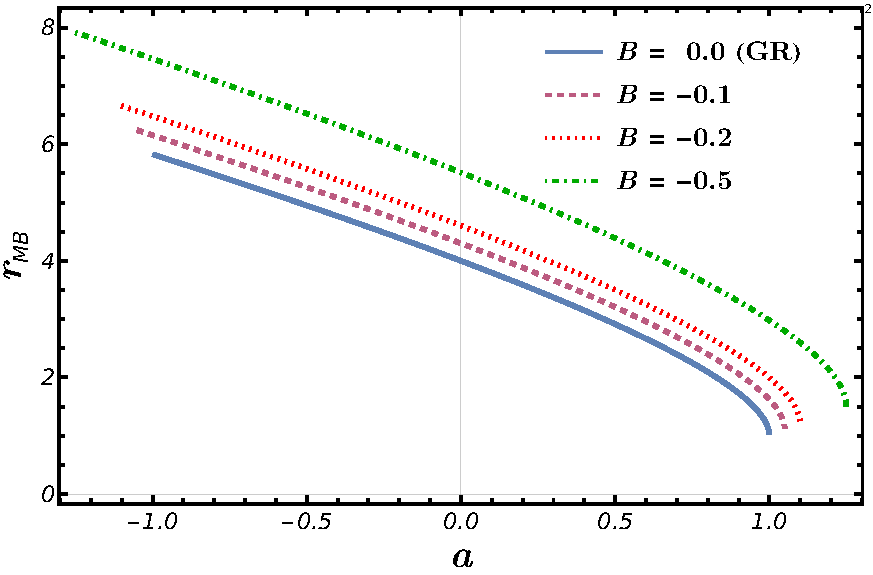
\includegraphics[width=0.7\textwidth]{r_MB_r_Vs_a.pdf}
    \caption{\centering Variation of marginally bound orbit as a function of spin of black hole for different $B$.}
    \label{r_MB_r_Vs_a}
\end{figure}
%%%% Image %%%%

%=========================================================
\section{Innermost stable circular orbit}
The innermost stable circular orbit (often called the ISCO) is the smallest marginally stable circular orbit, in which a test particle can stably orbit a massive body. To find the radius of ISCO, we opt for the same $V_{eff}$ as defined in the equation \Eref{Veff}. Since we are considering circular orbits, hence equation \Eref{14} is still valid. However, all the bound circular orbits are not stable. For stability condition, we must have the condition
\eq{ext}{\frac{{\partial }^2V_{eff}}{\partial r^2}\le 0.} 
The minimum radius (innermost radius) that satisfies all the three condition stated in equations \Eref{14} and \Eref{ext} is termed as Innermost Stable Circular Orbit (ISCO) and the radius named as $r_{ISCO}$. Numerically solving the three conditions simultaneously we obtain the variations of $r_{ISCO}$ shown in figure  \ref{r_ISCO_r_Vs_a}. Here we see a similar trend as of with $r_{mb}$, wee see that $r_{ISCO}$ increases with increasing $|B|$ and decreases with increasing $a$, and again the maximum value of $a$ have been modified and $B=0$ reproduces the results of GR.

%%%% Image %%%% 
\begin{figure}[H]
\centering
    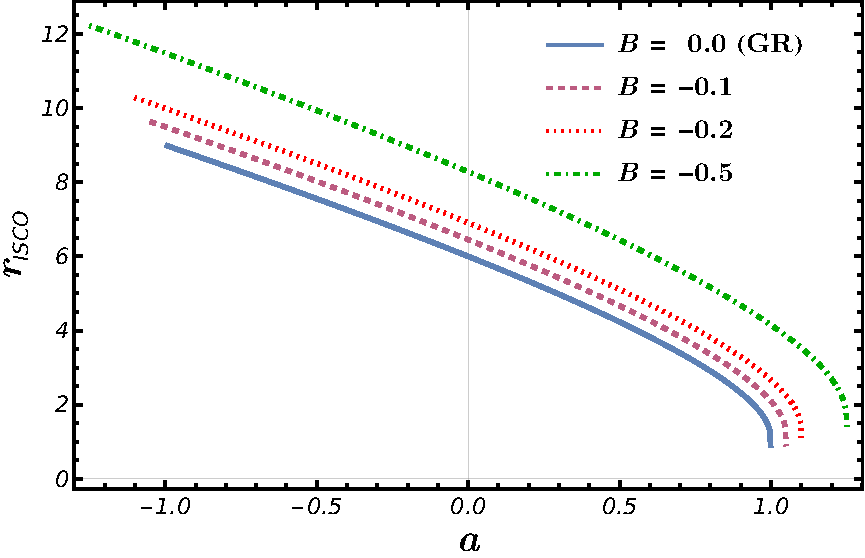
\includegraphics[width=0.7\textwidth]{r_ISCO_r_Vs_a.pdf}
    \caption{\centering Variation of marginally stable circular orbit as a function of spin of black hole for 
	different $B$.}
    \label{r_ISCO_r_Vs_a}
\end{figure}
%%%% Image %%%%


%=========================================================
\chapter{Epicyclic frequency in modified gravity}\label{Sec_Epi}
%%%% Image %%%% 
\begin{figure}[t]
	\begin{subfigure}[b]{0.5\textwidth}
         \centering
         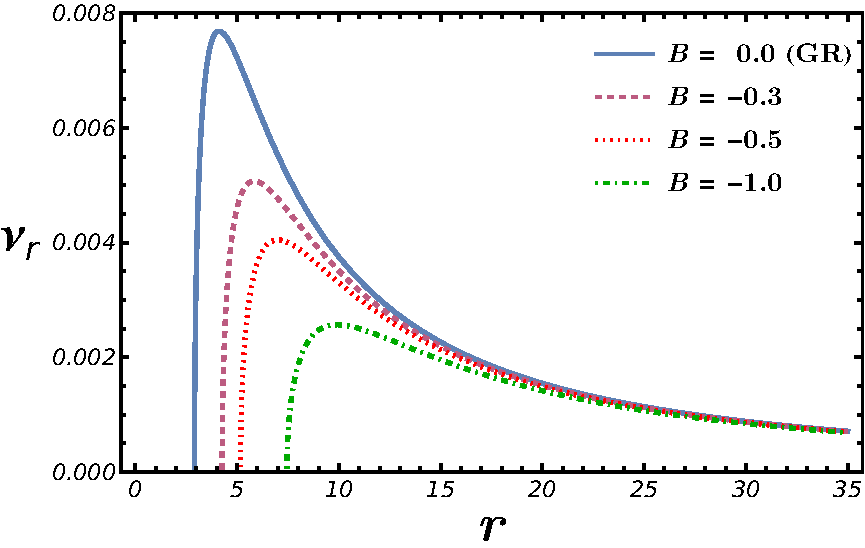
\includegraphics[width=0.8\textwidth]{nu_r_for_a_1.pdf}
	\caption{radial epicyclic frequencies $\nu_r$}
    		\label{nu_r_for_a_1}
     \end{subfigure}
    \hfill
     \begin{subfigure}[b]{0.5\textwidth}
         \centering
         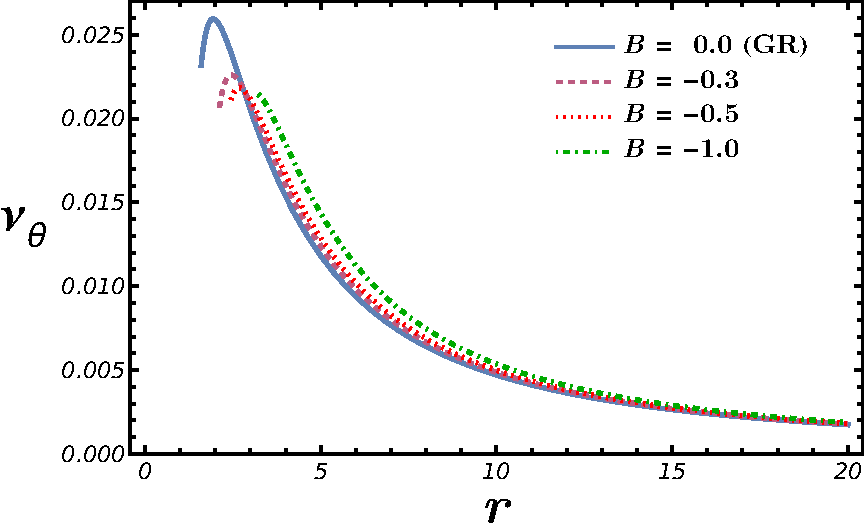
\includegraphics[width=0.8\textwidth]{nu_theta_for_a_1.pdf}
	\caption{vertical epicyclic frequencies $\nu_\theta$}
    		\label{nu_theta_for_a_1}
     \end{subfigure}
     \newline
	\newline
     \begin{subfigure}[b]{0.5\textwidth}
         \centering
         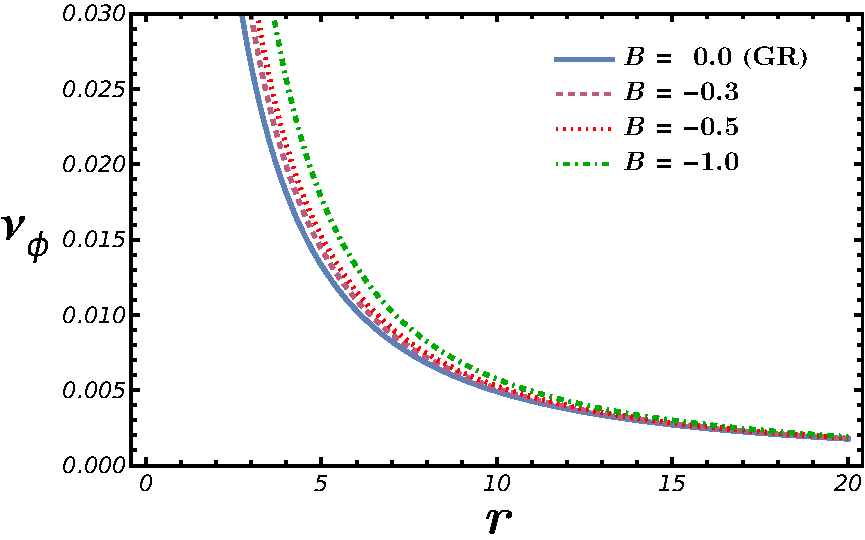
\includegraphics[width=0.8\textwidth]{nu_phi_for_a_1.pdf}
	\caption{orbital angular frequency $\nu_\varphi$}
    		\label{nu_phi_for_a_1}
     \end{subfigure}
 \begin{subfigure}[b]{0.5\textwidth}
         \centering
         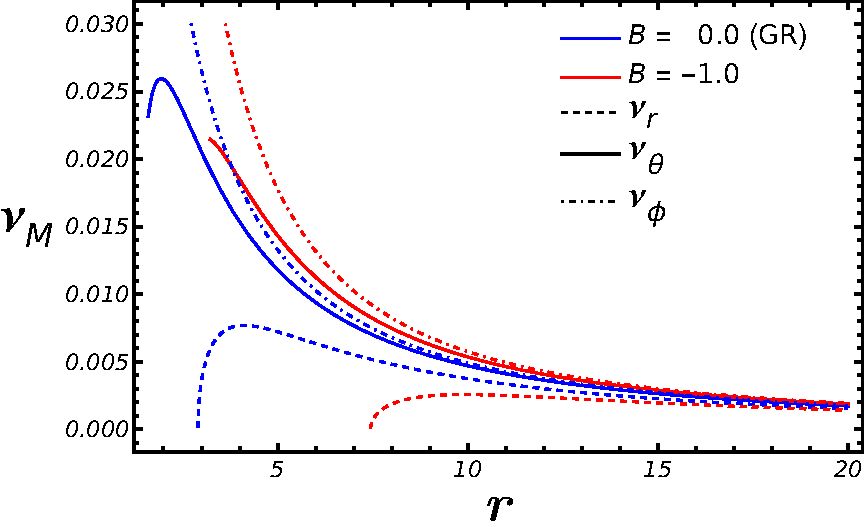
\includegraphics[width=0.8\textwidth]{Combine_Image.pdf}
	\caption{Comparison of various oscillation frequencies}
    		\label{nu_all_for_a_1}
     \end{subfigure}
        \caption{Profiles of the Keplerian frequency $\nu_\varphi$ and the epicyclic frequencies $\nu_r$ (radial) and $\nu_\theta$ (vertical) in the modified theory with spin parameter set to $a = 0.8$. The modified gravity parameter $B$ has been set to 0.0, -0.3, -0.5, -1.0 in (a), (b), and (c). In (d) $B=0$ and 
-1.0 for bottom and top curves respectively for $\nu_\varphi$ and $\nu_\theta$,
while for top and bottom curves for $\nu_r$.}
        \label{four graphs}
\end{figure}
%%%% Image %%%%
In this section we will briefly describe the derivation of epicyclic oscillation frequencies for the stationary, axisymmetric metric from the effective potential for circular geodesics, depicting the space-time around a rotating black hole. From equations \Eref{6}, \Eref{9}, \Eref{10} and \Eref{11} the line element can essentially be expressed as
\eq{line_element}{ds^2 = g_{tt}dt^2+2g_{t\varphi}dtd\varphi+g_{\varphi\varphi}d\varphi^2+g_{rr}dr^2+g_{\theta\theta}d\theta^2,} 
with $g_{\mu\nu}$ as a function of $r$ and $\theta$ and a symmetry along $\phi$
and $t$. It is most straightforward to obtain the epicyclic frequencies for a metric that can be expressed in this form. Epicyclic frequencies originate from the the relaxation of the circular orbits under external perturbation and it must be that this frequencies solely depend on the structure of the space-time around it. 


Now the similar normalization condition as in equation \Eref{u_normalize} along with equations \Eref{u_t} and \Eref{u_phi} but without a fixed $\theta$, hence with $u^\theta$, can be rewritten as 
\eq{u_normalize_new}{g_{rr}\left(u^r\right)^2+g_{\theta\theta}\left(u^\theta\right)^2 = \mathcal{V}_{eff},}
where the effective potential can be defined as
\eq{effective_potential_new}{\mathcal{V}_{eff} = \frac{\left(E^2-g_{tt}\right)g_{\varphi\varphi}+\left(2LE+g_{t\varphi}\right)g_{t\varphi}+L^2g_{tt}}{\left(g_{t\varphi}^2-g_{tt}g_{\varphi\varphi}\right)\Delta}.}
For circular orbits in the equatorial plane we have $u^r = u^\theta = 0$, which implies $\mathcal{V}_{eff} = 0$, and $\dot{u}^r = \dot{u}^\theta = 0$ give $\partial_r\mathcal{V}_{eff} = \partial_\theta\mathcal{V}_{eff} = 0$. From these 
three conditions $E$ and $L$ can be obtained as \cite{c_Bambi_12}
\eq{}{E = -\frac{g_{tt}+\Omega g_{t\varphi}}{\sqrt{-g_{tt}-2g_{t\varphi}\Omega-g_{\varphi\varphi}\Omega^2}},}

\eq{}{L = -\frac{g_{t\varphi}+\Omega g_{\varphi\varphi}}{\sqrt{-g_{tt}-2g_{t\varphi}\Omega-g_{\varphi\varphi}\Omega^2}}}
and the orbital angular frequency is given by \cite{c_Bambi_12}
\eq{Omega_varphi}{\Omega\equiv2\pi\nu_\varphi = \frac{-\partial_r g_{t\phi}\pm\sqrt{\left( \partial_rg_{t\varphi}\right)^2 - \partial_rg_{\varphi\varphi}\partial_rg_{tt}}}{\partial_rg_{\varphi\varphi}},}
where the positive (negative) sign in equation \Eref{Omega_varphi} refers to the co-rotating (counter-rotating) orbits with respect to the black hole spin. Equation 
\Eref{Omega_varphi} also defines the quantity $\nu_\varphi$ which is the frequency in which the particles move around the black hole in circular orbits.
Now the proper angular momentum ($\ell$) can be derived to be
\eq{curly_l}{\ell = -\frac{g_{t\varphi}+\Omega g_{\varphi\varphi}}{g_{tt}+\Omega g_{t\varphi}}.}

For finding the epicyclic frequencies, we first consider the perturbation to the radial $(r)$ and vertical $(\theta)$ 
coordinates so that \eq{per}{r(t)\approx r_0+\delta r(t)\text{,}\quad\theta(t)\approx \theta_0+\delta\theta(t),}
where the perturbations are considered to be $\delta r(t)\sim e^{i\Omega_rt}$ and $\delta\theta(t) \sim e^{i\Omega_\theta t}$, so as to have equations for harmonic oscillator of the form
\eq{radhar}{\frac{d^2\delta r}{dt^2} +\Omega_r^2\delta r = 0,}
\eq{anghar}{\frac{d^2\delta \theta}{dt^2} + \Omega_\theta^2\delta\theta = 0.}
Here  $r_0$ is the radius of the circular orbit and $\theta_0 = \pi/2$, is the angle at which the equatorial plane exists.
Now expanding the R.H.S. of equation \Eref{u_normalize_new} into second-order Taylor series along with the radial $(r)$ and vertical $(\theta)$ components,
replacing $r$ and $\theta$ from equation \Eref{per}, using equations \Eref{radhar} and \Eref{anghar}, 
and after some simple algebra made in appendix \ref{epi_calc} we obtain frequencies in equation \Eref{nu_r_appendix} and \Eref{nu_theta_appendix} as \cite{c_Bambi_12,Ryan}
\eq{nu_r}{\Omega_r^2 =\left(2\pi\nu_r\right)^2=- \frac{1}{2g_{rr}(u^t)^2}\frac{\partial^2\mathcal{V}_{eff}}{\partial r^2},}

\eq{nu_theta}{\Omega_\theta^2=\left(2\pi\nu_\theta\right)^2 =- \frac{1}{2g_{\theta\theta}(u^t)^2}\frac{\partial^2\mathcal{V}_{eff}}{\partial \theta^2}.}

The dependence of the frequencies on $B$ arises from various metric components. The explicit forms of the frequencies 
are huge and hence are not included in this work. Rather, we shall provide a numerical estimations of these frequencies. It should also be noted that these frequencies are observables and will be the key in estimating the most favored value of $B$ from observational data. 




The behaviors of $\nu_r$ and $\nu_\theta$ are shown in Figures \ref{nu_r_for_a_1} and \ref{nu_theta_for_a_1} with a fixed spin parameter $a = 0.8$. From Figure \ref{four graphs} it can be seen that $\nu_r$ decreases, while $\nu_\theta$ 
and $\nu_\phi$ increase, with the increase of $|B|$, at a given $r$ 
(particularly away from the black hole). However, the peak of $\nu_\theta$ 
decreases with increasing $|B|$. Also $\nu_r$ vanishes at a larger radius with
a smaller peak with increasing $|B|$. It can be easily seen from equation \Eref{Omega_varphi} that the GR result, i.e. $\Omega \sim (r^{3/2}\pm a)^{-1}$, can be found by setting $B=0$.



%========================================================= 
\chapter{Conclusion}
The idea of modification to gravity has been there in literature for some time, but its usefulness was not very clear. Although Starobinsky has used $R^2$- gravity to explain inflation \cite{1980PhLB...91...99S}, it was not clear if all the gravity theories are the same. In the last one decade or so, the authors
however, showed that $R^2$-gravity could be useful to sort out problems lying with
neutron stars and white dwarfs \cite{PhysRevD.82.064033,Arapo_lu_2011,
Upasana15,Kalita18} as well. However, none of this work has considered a black hole (vacuum) solution. After giving a brief introduction to modified $f(R)$ gravity, we first establish an asymptotically flat vacuum solution at first for non-rotating version giving rise to a modified Schwarzschild solution. Later we introduced rotation to the system using NJA. The solution mainly describes the space-time geometry around a rotating black hole, i.e., the modified Kerr black hole solution, for the first time of this kind to the best of our knowledge.

This work shows that depending on the modified gravity
parameter, all the fundamental properties of the black hole change, e.g., the 
radii of the black hole,
marginally stable, and bound circular orbits increase. Therefore, based on the
observed size, e.g., by the Event Horizon Telescope (EHT) image, the inference or
estimate of the spin of a black hole would be incorrect unless the proper theory is used.
If indeed, the gravity theory is based on an $f(R)$-gravity, the GR-based inference of the spin
of the black hole would actually underestimate it. This has many far-reaching
astrophysical implications.


While considering the approximate version of this solution with the modifications to gravity to be very small, then this solution exactly reproduces the results of black hole theories, which consider higher-dimensional branes \cite{Charged_BH_Brane, BH_Brane}. This work also showed both numerically and analytically (approximated) that this rotating solution allows the Kerr parameter to be greater than unity $a>1$ without forming any naked singularities. This naturally has important implications to the
cosmic censorship hypothesis \cite{1969NCimR...1..252P,2002GReGr..34.1141P}.
Therefore, black holes, according to this gravity theory, can spin faster without forming
naked singularity depending on the modified gravity parameter.

\appendix\label{Chap_Conclude}
\chapter{Einstein-Hilbert action and field equation}\label{A}
The Einstein-Hilbert action is given in equation \Eref{EH_action}, we can rewrite the equation by introducing a constant $\kappa$ as
\eq{}{S = \int \left[ \frac{1}{2\kappa}R + \mathcal{L}_M\right]\sqrt{-g}d^4x,}
where $\mathcal{L}_M$ is the matter Lagrangian.\\
Now from the principle of least action, we must have the variation of this action with respect to the inverse metric to be zero, yielding \cite{Sean,Misner_Thrones,M_Wald}
\aeq{A.2}{
\delta S =& 0\nonumber\\ 
=&\int\left[\frac{1}{2\kappa}\frac{\partial(\sqrt{-g}R)}{\delta g^{\mu\nu}}+\frac{\delta(\sqrt{-g}\mathcal{L}_M)}{\delta g^{\mu\nu}}\right]\nonumber\\
=&\int\left[\frac{1}{2\kappa}\left(\frac{\delta R}{\delta g^{\mu\nu}}+\frac{R}{\sqrt{-g}}\frac{\delta \sqrt{-g}}{\delta g^{\mu\nu}}\right)+\frac{1}{\sqrt{-g}}\frac{\delta(\sqrt{-g}\mathcal{L}_M)}{\delta g^{\mu\nu}}\right].
}
Now the last equation \Eref{A.2} is valid for any variation of $\delta g^{\mu\nu}$ and hence we can write
\eq{A.3}{\frac{1}{2\kappa}\left(\frac{\delta R}{\delta g^{\mu\nu}}+\frac{R}{\sqrt{-g}}\frac{\delta \sqrt{-g}}{\delta g^{\mu\nu}}\right)+\frac{1}{\sqrt{-g}}\frac{\delta(\sqrt{-g}\mathcal{L}_M)}{\delta g^{\mu\nu}}=0.}
From here we now define the energy-momentum tensor as
\eq{A.4}{T_{\mu\nu}:=\frac{-2}{\sqrt{-g}}\frac{\delta(\sqrt{-g}\mathcal{L}_M)}{\delta g^{\mu\nu}}=-2\frac{\delta \mathcal{L}_M}{\delta g^{\mu\nu}}+g_{\mu\nu}\mathcal{L}_M.}
%==================================================
\section{Variation of the metric determinant}
From Jacobi's formula we know the derivative of a determinant can be written as
\eq{}{d\det(A)=\operatorname {tr} (\operatorname {adj} (A)\,dA).}
And hence differentiation of the metric is of the form
\eq{}{\delta g=\delta \det(g_{\mu \nu })=gg^{\mu \nu }\delta g_{\mu \nu }.}
Here we could choose a coordinate system where the metric is in diagonal form and then apply the product rule to differentiate the product of factors on the main diagonal. Using this method we get,
\aeq{}{ \delta {\sqrt {-g}}&=-{\frac {1}{2{\sqrt {-g}}}}\delta g={\frac {1}{2}}{\sqrt {-g}}\left(g^{\mu \nu }\delta g_{\mu \nu }\right)\nonumber\\
&=-{\frac {1}{2}}{\sqrt {-g}}\left(g_{\mu \nu }\delta g^{\mu \nu }\right).}
Thus we conclude,
\eq{A.8}{{\frac {1}{\sqrt {-g}}}{\frac {\delta {\sqrt {-g}}}{\delta g^{\mu \nu }}}=-{\frac {1}{2}}g_{\mu \nu }.}

%==================================================
\section{Variation of Riemann tensor, Ricci tensor and Ricci scalar}
In differential geometry the Riemann tensor is the most common way used to express the curvature of Riemannian manifolds. It is expressed in terms of the Christoffel symbols as
\eq{}{R^{\rho }{}_{\sigma \mu \nu }=\partial _{\mu }\Gamma ^{\rho }{}_{\nu \sigma }-\partial _{\nu }\Gamma ^{\rho }{}_{\mu \sigma }+\Gamma ^{\rho }{}_{\mu \lambda }\Gamma ^{\lambda }{}_{\nu \sigma }-\Gamma ^{\rho }{}_{\nu \lambda }\Gamma ^{\lambda }{}_{\mu \sigma }.}
Now to calculate the variation of the Riemann tensor we first look at the variation of the Chistoffel symbols. Since $\delta \Gamma ^{\rho }{}_{\mu \sigma }$ is the difference of two connections, hence it is a tensor an we thus calculate its covariant derivative to be 
\eq{V_Chris}{\nabla _{\mu }\left(\delta \Gamma _{\nu \sigma }^{\rho }\right)=\partial _{\mu }(\delta \Gamma _{\nu \sigma }^{\rho })+\Gamma _{\mu \lambda }^{\rho }\delta \Gamma _{\nu \sigma }^{\lambda }-\Gamma _{\mu \nu }^{\lambda }\delta \Gamma _{\lambda \sigma }^{\rho }-\Gamma _{\mu \sigma }^{\lambda }\delta \Gamma _{\nu \lambda }^{\rho }.}
Now noting the variation of the Riemann tensor to be 
\eq{V_Riem}{\delta {R^{\rho }}_{\sigma \mu \nu }=\partial _{\mu }\delta \Gamma _{\nu \sigma }^{\rho }-\partial _{\nu }\delta \Gamma _{\mu \sigma }^{\rho }+\delta \Gamma _{\mu \lambda }^{\rho }\Gamma _{\nu \sigma }^{\lambda }+\Gamma _{\mu \lambda }^{\rho }\delta \Gamma _{\nu \sigma }^{\lambda }-\delta \Gamma _{\nu \lambda }^{\rho }\Gamma _{\mu \sigma }^{\lambda }-\Gamma _{\nu \lambda }^{\rho }\delta \Gamma _{\mu \sigma }^{\lambda },}
from equations \Eref{V_Chris} and \Eref{V_Riem} the expression of the variation of the Riemann tensor is the difference of two such terms as in equation \Eref{V_Chris} and hence
\eq{}{\delta {R^{\rho }}_{\sigma \mu \nu }=\nabla _{\mu }\left(\delta \Gamma _{\nu \sigma }^{\rho }\right)-\nabla _{\nu }\left(\delta \Gamma _{\mu \sigma }^{\rho }\right).}
Contracting two indices we obtain the Palantini's identity 
\eq{}{\delta R_{\sigma \nu }\equiv \delta {R^{\rho }}_{\sigma \rho \nu }=\nabla _{\rho }\left(\delta \Gamma _{\nu \sigma }^{\rho }\right)-\nabla _{\nu }\left(\delta \Gamma _{\rho \sigma }^{\rho }\right),}
and from the definition of the Ricci Scala $R = g^{\sigma\nu}R_{\sigma\nu}$, the variation to Ricci scalar is given by
\aeq{}{\delta R&=R_{\sigma \nu }\delta g^{\sigma \nu }+g^{\sigma \nu }\delta R_{\sigma \nu }\nonumber\\&=R_{\sigma \nu }\delta g^{\sigma \nu }+\nabla _{\rho }\left(g^{\sigma \nu }\delta \Gamma _{\nu \sigma }^{\rho }-g^{\sigma \rho }\delta \Gamma _{\mu \sigma }^{\mu }\right).}
The last term,$\nabla _{\rho }\left(g^{\sigma \nu }\delta \Gamma _{\nu \sigma }^{\rho }-g^{\sigma \rho }\delta \Gamma _{\mu \sigma }^{\mu }\right)$, i.e. $\nabla _{\rho }A^{\rho }\equiv A^{\lambda }{}_{;\lambda } \nabla _{\rho }A^{\rho }\equiv A^{\lambda }{}_{;\lambda }$, with $ A^{\rho }=g^{\sigma \nu }\delta \Gamma _{\nu \sigma }^{\rho }-g^{\sigma \rho }\delta \Gamma _{\mu \sigma }^{\mu }$,
multiplied by $\sqrt{-g}$ becomes a total derivative, now since for any vector $A^{\lambda}$ and any tensor density $\sqrt{-g}A^{\lambda}$ we have,
\eq{}{ {\sqrt {-g}}\,A_{;\lambda }^{\lambda }=({\sqrt {-g}}\,A^{\lambda })_{;\lambda }=({\sqrt {-g}}\,A^{\lambda })_{,\lambda }.}
Now by stokes theorem, we obtain a boundary term when this is integrated. This boundary term is, in general non-zero. However, when the variation of the metric $\delta g^{\mu\nu}$ vanishes in a neighbourhood of the boundary or when there is no boundary, this term does not contribute to the variation of the action, And thus at events not in the closure of the boundary, we obtain
\eq{A.16}{{\frac {\delta R}{\delta g^{\mu \nu }}}=R_{\mu \nu }.}
 
%=====================================================
\section{Einstein's field equations}\label{A_EF_Eq}
Now from the previous section we know the variation of various elements. Hence from equations \Eref{A.3}, \Eref{A.4}, \Eref{8} and \Eref{A.16} the equation of motion turns out to be 
\eq{}{ R_{\mu \nu }-{\frac {1}{2}}g_{\mu \nu }R={\frac {8\pi G}{c^{4}}}T_{\mu \nu },}
putting the value of $\kappa = \frac{8\pi G}{c^4}$ we obtain the Einstein's field equations as
\eq{App_Field_eq}{G_{\mu\nu} = R_{\mu\nu}-\frac{1}{2}g_{\mu\nu}R = \frac{8\pi G}{c^4}T_{\mu\nu}.}

%======================================================
%======================================================
\chapter{Field equations in $f(R)$ gravity}
In $f(R)$ one seeks to generalise the Lagrangian of the Einstein-Hilbert action equation \Eref{EH_action} so as the Ricci scalar is replaced with an arbitrary function of $R$. The resulting equation is of the form as in equation \Eref{mod_action}, defining $\kappa$ as in \ref{A} the gravitational part of modified action is of the form
\eq{}{S[g]=\int {1 \over 2\kappa }f(R){\sqrt {-g}}\,\mathrm {d} ^{4}x.}
Now, referring to equations \Eref{A.3}, \Eref{A.4}, \Eref{8} and \Eref{A.16} the variation of the action is calculated as
\aeq{}{
\delta S[g]&=\int {\frac {1}{2\kappa }}\left(\delta f(R){\sqrt {-g}}+f(R)\delta {\sqrt {-g}}\right)\,
\mathrm {d} ^{4}x\\&=\int {\frac {1}{2\kappa }}\left(F(R)\delta R{\sqrt {-g}}-{\frac {1}{2}}{\sqrt {-g}}g_{\mu \nu }\delta g^{\mu \nu }f(R)\right)\,\mathrm {d} ^{4}x
\\&=\int {\frac {1}{2\kappa }}{\sqrt {-g}}\left[F(R)(R_{\mu \nu }\delta g^{\mu \nu }+g_{\mu \nu }\Box \delta g^{\mu \nu }-\nabla _{\mu }\nabla _{\nu }\delta g^{\mu \nu })\right.\nonumber
\\&\hspace{5cm}\left.-{\frac {1}{2}}g_{\mu \nu }\delta g^{\mu \nu }f(R)\right]\,\mathrm {d}
^{4}x.}
Doing integration by parts of the second and the third term and neglecting the boundary contribution we arrive at
\eq{}{ \delta S[g]=\int {\frac {1}{2\kappa }}{\sqrt {-g}}\delta g^{\mu \nu }\left(F(R)R_{\mu \nu }-{\frac {1}{2}}g_{\mu \nu }f(R)+[g_{\mu \nu }\Box -\nabla _{\mu }\nabla _{\nu }]F(R)\right)\,\mathrm {d} ^{4}x.}
Now the variation should be zero for any variation in $\delta g^{\mu \nu }$, hence we get the modified field equations to be
\eq{}{ F(R)R_{\mu \nu }-{\frac {1}{2}}f(R)g_{\mu \nu }+\left[g_{\mu \nu }\Box -\nabla _{\mu }\nabla _{\nu }\right]F(R)=\kappa T_{\mu \nu },}
where the energy momentum tensor is defined as in equation \Eref{A.4}


%======================================================
%======================================================
\chapter{Expression for epicyclic frequency}\label{epi_calc}

Here we consider a test particle moving in a circular orbit at some radius $r_0$ and at some angle $\theta_0$. For finding the epicyclic frequencies we first consider a perturbation to the radial$ (r)$ and vertical $(\theta)$ 
components so that
\eq{}{r(t)\approx r_0+\delta r(t)\text{,}\quad\theta(t)\approx \theta_0+\delta\theta(t),}
where the perturbation are considered to be $\delta r(t)\sim e^{i\Omega_rt}$ and $\delta\theta(t) \sim e^{i\Omega_\theta t}$, so as to have a wave equation of the form
\eq{}{\frac{d^2\delta r}{dt^2} +\Omega_r^2\delta r = 0,}
\eq{}{\frac{d^2\delta \theta}{dt^2} + \Omega_\theta^2\delta\theta = 0.}
From equation \Eref{u_normalize_new}, the relation between the effective potential and $u^r$ and $u^\theta$ is
\[g_{rr}\left(u^r\right)^2+g_{\theta\theta}\left(u^\theta\right)^2 = \mathcal{V}_{eff}.\]

\noindent The right-hand side of this equation can be expanded into second-order Taylor series along with the radial $(r)$ and vertical $(\theta)$ component. Note that in this consideration $\delta r(t)\equiv$ radial perturbation to the value of $r$ which along $\theta = \pi/2$, maximizes the right hand side, similar consideration have made for $\delta \theta$. The vanishing of the mixed $r\theta$ derivative comes from the reflection symmetry implying the motion in $r$ and $\theta$ directions are independent of each other. Thus the Taylor expansion becomes
\eq{Taylor}{ \mathcal{V}_{eff}\approx  \left(\mathcal{V}_{eff}\right)_{r_0,\theta_0} + \frac{1}{2}\left(\delta r\right)^2\left(\frac{\partial^2\mathcal{V}_{eff}}{\partial r^2}\right)_{r_0,\theta_0} +  \frac{1}{2}\left(\delta\theta\right)^2\left(\frac{\partial^2\mathcal{V}_{eff}}{\partial \theta^2}\right)_{r_0,\theta_0}.}
On the other hand the right side of the equation \Eref{u_normalize_new} can be written as
\eq{again_u_normalize_new}{g_{rr}\left(u^r\right)^2+g_{\theta\theta}\left(u^\theta\right)^2 = g_{rr}\left(u^t\right)^2\left(\frac{d \delta r}{dt}\right)^2+g_{\theta\theta}\left(u^t\right)^2\left(\frac{d \delta \theta}{dt}\right)^2.}
Now from the equations \Eref{u_normalize_new}, \Eref{Taylor} and \Eref{again_u_normalize_new} we arrive at
\meq{2D_HO}{ \left[g_{rr}\left(u^t\right)^2\left(\frac{d \delta r}{dt}\right)^2 - \frac{1}{2}\left(\delta r\right)^2\left(\frac{\partial^2\mathcal{V}_{eff}}{\partial r^2}\right)_{r_0,\theta_0}\right] \\+\left[ g_{\theta\theta}\left(u^t\right)^2\left(\frac{d \delta \theta}{dt}\right)^2 - \frac{1}{2}\left(\delta\theta\right)^2\left(\frac{\partial^2\mathcal{V}_{eff}}{\partial \theta^2}\right)_{r_0,\theta_0}\right] = \left(\mathcal{V}_{eff}\right)_{r_0,\theta_0}. }
This can be identified as the energy conservation equation of a two-dimensional harmonic oscillator, and hence the corresponding angular frequencies can be found to be
\eq{nu_r_appendix}{\Omega_r^2 =- \frac{1}{2g_{rr}(u^t)^2}\left(\frac{\partial^2\mathcal{V}_{eff}}{\partial r^2}\right)_{r_0,\theta_0},}
and 
\eq{nu_theta_appendix}{\Omega_\theta^2 =- \frac{1}{2g_{\theta\theta}(u^t)^2}\left(\frac{\partial^2\mathcal{V}_{eff}}{\partial \theta^2}\right)_{r_0, \theta_0}.}

\printbibliography





\end{document}






%This things will not get included in the main material
\begin{titlepage}
    \begin{center}
            
        \LARGE
        \textbf{Asymptotically flat vacuum solution for a rotating black hole in a modified 
gravity theory}
            
        \vspace{0.5cm}
 
        A Thesis submitted for the completion of requirements for the degree of\\
        \vspace{0.8cm}
        \LARGE
        \textbf{Bachelor of Science (Research)}\\
        \vspace{0.8cm}
        by
        \vspace{0.8cm}
            
        \textbf{Arghya Ranjan Das}\\
        Undergraduate Programme\\
        Indian Institute of Science

        
\includegraphics[width=0.4\textwidth]{University_logo.pdf}

            
        \Large
        Under the supervision of\\
        Prof. Banibrata Mukhopadhyay\\
        Department of Physics, Indian Institute of Science
        
            
    \end{center}
\end{titlepage}